% This is file JFM2esam.tex
% first release v1.0, 20th October 1996
%       release v1.01, 29th October 1996
%       release v1.1, 25th June 1997
%       release v2.0, 27th July 2004
%       release v3.0, 16th July 2014
%   (based on JFMsampl.tex v1.3 for LaTeX2.09)
% Copyright (C) 1996, 1997, 2014 Cambridge University Press

\documentclass{jfm}
\usepackage{graphicx}
\usepackage{epstopdf, epsfig}
\usepackage{amsmath}
\usepackage{amsfonts}
\newtheorem{lemma}{Lemma}
\newtheorem{corollary}{Corollary}

% our colors
\usepackage[usenames,dvipsnames]{xcolor}
\colorlet{cesar}{red}
\colorlet{greg}{green}
\colorlet{bill}{blue}

% copy-editing printing
% \usepackage{geometry}
% \geometry{a4paper,left=5.25cm,right=5 .25cm,top=3.5cm,bottom=3.5cm}
% \linespread{1.}
% \usepackage{multicol}


% our packages
\usepackage{showlabels}

% hyperref
\usepackage{hyperref}
\hypersetup{
        %draft,
        breaklinks=true,
        colorlinks=true,
        linkcolor=blue,
        citecolor=Purple,
        urlcolor=Purple,
        pdfstartview={FitH},
        pdfview={FitH 0},
        pdfauthor={Cesar B. Rocha},
        pdftitle={stimulated generation},
 }


\newcommand{\NIW}{near-inertial wave}
\newcommand{\macrot}{macroturbulence}

%\shorttitle{ Extraction of  energy from barotropic turbulence by near-inertial waves}
\shorttitle{Stimulated generation}

\shortauthor{Cesar B. Rocha, Gregory L. Wagner, and William R Young}

%\title{Extraction of energy from quasi-gestrophic flow by near-inertial waves:\\
%        stimulated generation}
\title{Stimulated generation: extraction of energy from balanced flow
       by near-inertial waves}


%\title{Near-inertial waves extract energy from barotropic quasi-geostrophic flow}
\author{Cesar B. Rocha\aff{1}
  \corresp{\email{crocha@ucsd.edu}},
  Gregory L. Wagner\aff{2}
 \and William R. Young\aff{1}}

\affiliation{\aff{1}Scripps Institution of Oceanography, University of California,
            San Diego
\aff{2}Department of Earth, Atmospheric and Planetary Sciences, Massachusetts
            Institute of Technology}



\begin{document}

\newcommand{\com}{\, ,}
\newcommand{\per}{\, .}

%% Averages
% Use \bar to over line solo symbols

\newcommand{\av}[1]{\bar{#1}}
\newcommand{\avbg}[1]{\overline{#1}}
\newcommand{\avbgg}[1]{\overline{#1}}

% A nice definition
\newcommand{\defn}{\ensuremath{\stackrel{\mathrm{def}}{=}}}

% space in equations
\newcommand{\qqand}{\qquad \text{and} \qquad}
\newcommand{\qand}{\quad \text{and} \quad}

% equations
\def\beq{\begin{equation}}
\def\eeq{\end{equation}}

\def\bea{\begin{align}}
\def\ena{\end{align}}


% calculus
\newcommand{\ord}{\mathcal{O}}
%\newcommand{\p}{\partial}
\newcommand{\ii}{{\rm i}}
\newcommand{\dd}{{\rm d}}
\newcommand{\id}{{\, \rm d}}
\newcommand{\ee}{{\rm e}}
\newcommand{\DD}{{\rm D}}
\newcommand{\wavy}{\text{wavy}}
\newcommand{\qg}{\text{qg}}
\newcommand{\dt}{\Delta t}
\newcommand{\dx}{\Delta x}
\newcommand{\be}{\beta}

\newcommand{\al}{\alpha}
\newcommand{\bx}{\boldsymbol{x}}
\newcommand{\by}{\boldsymbol{y}}
\newcommand{\bu}{\boldsymbol{u}}
\newcommand{\bv}{\boldsymbol{v}}


\newcommand{\half}{\tfrac{1}{2}}
\newcommand{\halfi}{\tfrac{\ii}{2}}
\newcommand{\quarter}{\tfrac{1}{4}}
\newcommand{\quarteri}{\tfrac{\ii}{4}}
\newcommand{\halfrho}{\tfrac{1}{2}}
\newcommand{\rz}{{}}
\newcommand{\bn}{\boldsymbol{\hat n}}
\newcommand{\br}{\boldsymbol{r}}
\newcommand{\bR}{\boldsymbol{R}}
\newcommand{\bA}{\ensuremath {\boldsymbol {A}}}
\newcommand{\bB}{\ensuremath {\boldsymbol {B}}}
\newcommand{\bU}{\ensuremath {\boldsymbol {U}}}
\newcommand{\bE}{\ensuremath {\boldsymbol {E}}}
\newcommand{\bN}{\ensuremath {\boldsymbol {\mathrm{N}}}}
\newcommand{\bJ}{\ensuremath {\boldsymbol {J}}}
\newcommand{\bXX}{\ensuremath {\boldsymbol {\mathcal{X}}}}
\newcommand{\bFF}{\ensuremath {\boldsymbol {F}}}
\newcommand{\bF}{\ensuremath {\boldsymbol {F}^{\sharp}}}
\newcommand{\bG}{\ensuremath {\boldsymbol G}}
\newcommand{\bSigma}{\ensuremath {\boldsymbol {\Sigma}}}
\newcommand{\bvarphi}{\ensuremath {\boldsymbol {\varphi}}}
\newcommand{\bxi}{\ensuremath {\boldsymbol {\xi}}}
\newcommand{\avbxi}{\overline{\ensuremath {\boldsymbol {\xi}}}}

% math cal

\newcommand{\J}{\mathcal{J}}
\newcommand{\K}{\mathcal{K}}
\newcommand{\cG}{\mathcal{G}}
\newcommand{\cF}{\mathcal{F}}
\newcommand{\cN}{\mathcal{N}}
\newcommand{\cL}{\mathcal{L}}
\newcommand{\cS}{\mathcal{S}}
\newcommand{\cE}{\mathcal{E}}


% san serif for matrices and differential operators
%\newcommand{\helmn}{\mathsf{H}_n}
\newcommand{\helmm}{\triangle_m}
\newcommand{\helmn}{\triangle_n}
\newcommand{\helms}{\triangle_s}
\newcommand{\helm}{\triangle}
\newcommand{\sA}{\mathsf{A}}
\newcommand{\sB}{\mathsf{B}}
\newcommand{\sG}{\mathsf{G}}
\newcommand{\sI}{\mathsf{I}}
%\newcommand{\sJ}{\mathsf{J}}
\newcommand{\sJ}{J}
\newcommand{\gsJ}{\breve{\mathsf{J}}}
\newcommand{\sU}{\mathsf{U}}
\newcommand{\sP}{\mathsf{P}}
\newcommand{\sQ}{\mathsf{Q}}
\newcommand{\sR}{\mathsf{R}}
\newcommand{\sL}{\mathsf{L}}
\newcommand{\Lu}{\mathsf{L}(\what{u}_k)}
\newcommand{\Nu}{\mathsf{N}(\what{u}_k)}
\renewcommand{\L}{\mathsf{L}}
\newcommand{\N}{\mathsf{N}}
\newcommand{\sH}{\mathsf{H}}
\renewcommand{\sI}{\mathsf{I}}
\renewcommand{\L}{\mathsf{L}}
\newcommand{\sM}{\mathsf{M}}
\newcommand{\sT}{\mathsf{T}}
\newcommand{\sGamma}{\mathsf{\Gamma}}
\newcommand{\sOmega}{\mathsf{\Omega}}
\newcommand{\sSigma}{\mathsf{\Omega}}
\newcommand{\sbeta}{\mathsf{\beta}}
\newcommand{\sPi}{\mathsf{\Pi}}
\newcommand{\sC}{\mathsf{C}}
\newcommand{\sQy}{\mathsf{Q}}
\renewcommand{\sb}{\mathsf{b}}

% u
\newcommand{\uhat}{\what{u}_k}

% angle brackets

\def\la{\langle}
\def\ra{\rangle}
\def\laa{\left \langle}
\def\raa{\right \rangle}


%grads and div's
%\newcommand{\bcdot}{\hspace{-0.1em} \boldsymbol{\cdot} \hspace{-0.12em}}
%\newcommand{\bnabla}{\boldsymbol{\nabla}}
\newcommand{\bnablaH}{\bnabla_{\! \mathrm{h}}}
\newcommand{\grad}{\bnabla}
\newcommand{\gradH}{\bnablaH}
\newcommand{\curl}{\bnabla \!\times\!}
\newcommand{\diver}{\bnabla \! \bcdot \! }
\newcommand{\cross}{\times}
%\newcommand{\lap}{\nabla^2}
\newcommand{\lap}{\triangle}

%varthetas and thetas
\newcommand{\vth}{\vartheta}
\newcommand{\psii}{\psi^{\mathrm{i}}}
\newcommand{\thb}{\theta^{\mathrm{-}}}
\newcommand{\vthb}{\vartheta^{\mathrm{-}}}
\newcommand{\vthbhat}{{\hat{\vartheta}}^{\mathrm{-}}}
\newcommand{\vThb}{\varTheta^{\mathrm{-}}}
\newcommand{\psib}{\psi^{\mathrm{-}}}
\newcommand{\tht}{\theta^{\mathrm{+}}}
\newcommand{\vtht}{\vartheta^{\mathrm{+}}}
\newcommand{\vththat}{{\hat{\vartheta}}^{\mathrm{+}}}
\newcommand{\vthtbhat}{{\hat{\vartheta}}^{\pm}}
\newcommand{\vTht}{\varTheta^{\mathrm{+}}}
\newcommand{\vthtb}{\vartheta^{\pm}}
\newcommand{\vThtb}{\varTheta^{\pm}}

% nondimensional numbers
\renewcommand{\Re}{\mathrm{Re}}
\newcommand{\Ro}{\mathrm{Ro}}
\newcommand{\Bu}{\mathrm{Bu}}
\newcommand{\Ri}{\mathrm{Ri}}

%psi's
%Galerking coefficient for psi:
\newcommand{\gpsi}{\breve \psi}
\newcommand{\gpsic}{{\breve \psi}^\star}
\newcommand{\gtau}{\breve \tau}
\newcommand{\gtauc}{{\breve \tau}^\star}
\newcommand{\gphi}{\breve \phi}
\newcommand{\gq}{\breve q}
\newcommand{\gU}{\breve U}
\newcommand{\gQ}{\breve Q}
\newcommand{\gsigma}{\breve \sigma}


\newcommand{\psit}{\psi^{\mathrm{+}}}
\newcommand{\psithat}{{\hat{\psi}}^{\mathrm{+}}}
\newcommand{\psibhat}{{\hat{\psi}}^{\mathrm{-}}}
\newcommand{\psitb}{\psi^{\pm}}
\newcommand{\psitbhat}{{\hat{\psi}}^\pm}
\newcommand{\St}{S^{\mathrm{+}}}
\newcommand{\Sb}{S^{\mathrm{-}}}
\newcommand{\phb}{\phi^{\mathrm{-}}}
\newcommand{\pht}{\phi^{\mathrm{+}}}
\newcommand{\tautb}{\tau^{\pm}}
\newcommand{\sigmatb}{\sigma^{\pm}}


\newcommand{\bur}{\left(\tfrac{f_0}{N}\right)^2}
\newcommand{\ibur}{\left(\tfrac{N}{f_0}\right)^2}
\newcommand{\Nm}{N_{\mathrm{mix}}}
\newcommand{\xim}{\xi_{\mathrm{mix}}}
\newcommand{\hs}{h_*}
\renewcommand{\sp}{\mathsf{p}}
\newcommand{\se}{\mathsf{e}}
\newcommand{\sptb}{\mathsf{p}^\pm}


%nmax is a problem:
%\newcommand{\nmax}{n_{\mathrm{max}}}
\newcommand{\nmax}{\mathrm{N}}
\newcommand{\mmax}{\mathrm{M}}

\newcommand{\WKB}{\mathrm{WKB}}
\newcommand{\Lam}{\Lambda}
\newcommand{\tha}{\theta}
\newcommand{\kap}{\kappa}
\newcommand{\bphi}{\boldsymbol{\phi}}
\newcommand{\third}{\tfrac{1}{3}}
\newcommand{\cs}{c^\star}
\newcommand{\dstar}{{\star\star}}
\newcommand{\nt}{n^{\mathrm{trnc}}}
\newcommand{\sDp}{\mathsf{D}^1_{\nmax}}
\newcommand{\sDpp}{\mathsf{D}^2_{\nmax}}
\newcommand{\sD}{\mathsf{D}}
\newcommand{\sDN}{\mathsf{D_\nmax}}
\newcommand{\sK}{\mathsf{K_2}}
\newcommand{\stheta}{\mathsf{\theta}}
\newcommand{\sphi}{\mathsf{\phi}}
\newcommand{\sq}{\mathsf{q}}
\newcommand{\cosech}{\text{csch}\,}
\newcommand{\sinc}{\text{sinc}\,}

%%%%%%%%% %%%%

%%%%%%%%% %%%%
\newcommand{\zt}{z^+}
\newcommand{\zb}{z^-}
\newcommand{\qA}{q^A_{\nmax}}
\newcommand{\psiB}{\psi^B_{\nmax}}
\newcommand{\phiB}{\phi^B_{\nmax}}
\newcommand{\eye}{\boldsymbol{\hat{i}}}
\newcommand{\jay}{\boldsymbol{\hat{j}}}
\newcommand{\kay}{\boldsymbol{\hat{k}}}
\newcommand{\psiG}{\psi^{\mathrm{G}}}
\newcommand{\qG}{q^{\mathrm{G}}}
\newcommand{\uG}{u^{\mathrm{G}}}
\newcommand{\UG}{U^{\mathrm{G}}}
\newcommand{\UGN}{U^{\mathrm{G}}_{\nmax}}
\newcommand{\QGN}{Q^{\mathrm{G}}_{\nmax}}
\newcommand{\sumoddn}{\sum_{n = 1, n~ \text{odd}}^{\nmax}}

% bretherton
\newcommand{\qBr}{q_{\mathrm{Br}}}
\newcommand{\psiBr}{\psi_{\mathrm{Br}}}

\newcommand{\ep}{\epsilon}
\newcommand{\vep}{\varepsilon}


%\renewcommand{\sZ}{\mathsf{Z}}
%\renewcommand{\sE}{\mathsf{E}}
\newcommand{\iBu}{\left(\tfrac{f_0}{N}\right)^2}
\newcommand{\F}{\mathcal{F}}
\newcommand{\D}{\mathcal{D}}
\newcommand{\phis}{\phi^\star}

\newcommand{\Sf}{\mathbf{S}}
\newcommand{\ut}{\mathbf{u}^\#}
\newcommand{\cg}{\mathbf{c}_g}
\newcommand{\Uf}{\mathbf{U}}
\renewcommand{\Im}{\mathrm{Im}}
\renewcommand{\div}{\nabla\cdot}
\renewcommand{\P}{\mathcal{P}}
\newcommand{\dU}{\delta U}
\newcommand{\W}{\mathcal{W}}
\newcommand{\cK}{\mathcal{K}}
\newcommand{\cP}{\mathcal{P}}
\renewcommand{\L}{\mathsf{L}}
\renewcommand{\N}{\mathsf{N}}
\newcommand{\psiq}{\psi^q}
\newcommand{\psiw}{\psi^w}
%\newcommand{\tfrac}{\frac}
%\newcommand{\eqref}{\ref}
\newcommand{\kb}{\mathbf{k}}
\newcommand{\xb}{\mathbf{x}}
%wave PV
\newcommand{\qw}{q^{\mathrm{w}}}
\newcommand{\bw}{b^{\mathrm{w}}}
\newcommand{\ug}{u^{\mathrm{g}}}
\newcommand{\bug}{\bu^{\mathrm{g}}}

%action and energy
\newcommand{\A}{  \mathcal{A}}
\newcommand{\E}{\mathcal{E}}
\newcommand{\Pw}{\mathcal{P}}
\newcommand{\Ke}{\mathcal{K}}
\newcommand{\Ff}{ \boldsymbol{\mathcal{F}}}
\newcommand{\Ffp}{\boldsymbol{\mathcal{F}}^{\perp}}
\newcommand{\Hf}{\boldsymbol{\mathcal{H}}}
\newcommand{\Gg}{\boldsymbol{\mathcal{G}}}
\newcommand{\epA}{\varepsilon_\mathcal{A}}
\newcommand{\epP}{\varepsilon_\mathcal{P}}
\newcommand{\epK}{\varepsilon_\mathcal{K}}

%dispersivity
\newcommand{\disp}{\eta}

% index differentiation
\newcommand{\gind}[2]{#1_{,#2}}


\maketitle

\begin{abstract}
\end{abstract}

\begin{keywords}

\end{keywords}


\section{Introduction}

% 1) The mesoscale energy conundrum: a recalcitrant problem
The  inverse cascade, acting on balanced ocean \macrot{},  transfers energy towards
large spatial scales. But a statistically steady ocean circulation requires
energy dissipation at the same rate as it is supplied  by wind.  Thus equilibration of
the  ocean \macrot{}  requires ageostrophic processes, acting in opposition to the
inverse cascade, to produce   a transfer of energy  towards the centimeter scales
at which molecular viscosity is effective.  Mechanisms that might result in this
down-scale transfer   include, but are not limited to, surface and
benthic boundary-layer turbulence, lee-wave generation by mesoscale eddies negotiating
bottom topography, and the spontaneous generation of internal waves by upper-ocean
frontal instabilities; see the introduction of \citet{nagai_etal2015} for a recent
review. Here we focus on a mechanism first identified  in a modeling study by
\cite{gertz_straub2009}:  externally forced \NIW s might provide an energy sink
for large-scale balanced flow. Since \cite{gertz_straub2009}, several other studies,
summarized in table \ref{modelzTable}, have argued for significant energy transfer
to \NIW s from balanced flows.

Using the generalized  Lagrangian mean formulation,  \citet{xie_vanneste2015}
(XV hereafter) developed a phase-averaged model for the interaction between \NIW
s and slowly evolving  balanced flow. Alternative derivations of the  XV model with  different
scaling assumptions  have been provided by \cite{salmon2016} and \cite{wagner_young2016}. The conservation laws of the XV model  qualitatively explain  the energy transfers identified by the papers in table \ref{modelzTable}. To distinguish this mechanism from \textit{spontaneous} generation, and to complete an electromagnetic analogy, XV refer to the transfer of energy from balanced flow to externally forced near-inertial waves  as  \textit{stimulated} generation.  Alternative terms to stimulated generation  used in the  literature are  summarized in  table \ref{modelzTable}.
The diversity of  studies in table \ref{modelzTable} indicates that stimulated
generation is a common, and therefore probably  important, wave mean flow interaction.

Stimulated generation is a consequence of the reduction in \NIW{} length scales
resulting from  advection and refraction of \NIW s by the balanced flow.
Stimulated generation should be contrasted with the more widely studied process
of spontaneous generation, which is the emission of internal waves arising
from the slow evolution of balanced flow in the absence  of external forcing at
wave frequencies \citep{vanneste2013}. Spontaneous generation is inefficient at
small and  moderate Rossby numbers and its global impact on the energetics of the
ocean \macrot{}   is probably small \citep{danioux_etal2012, nagai_etal2015}.
Spontaneous generation is localized at sharp submeoscale fronts with  order one
Rossby  number   \citep[e.g., ][]{shakespeare_hogg2017} while the stimulated variety  operates even at  small Rossby numbers characteristic of most interior oceanic conditions, provided only that internal waves are introduced by external forcing. 

\begin{table}
\label{modelzTable}
\caption{Summary of model-based studies of energy extraction from balanced flow by near-inertial waves.}
  \begin{center}
     \begin{tabular}{ p{.285\textwidth} p{.4\textwidth} |   p{.3\textwidth}    }
     %\begin{tabular}{ c  p{.4\textwidth} l p{0.2\textwidth} }
       \hline
         Study &  Framework &   \textit{Stimulated generation} is referred to as \\ \hline
   \cite{gertz_straub2009} & {Barotropic 2D double-gyre solutions coupled with forced 3D
                              near-inertial waves.}
                              & \textit{2D--to--3D energy transfer}
                              \\ \hline
 \cite{thomas_2012} & {Near-inertial waves in a baroclinic geostrophic flow undergoing frontogenesis.}
                              & \textit{deformation shear production}
                              \\ \hline
    \cite{whitt_thomas2015}  & Mixed-layer slab model modified by geostrophic
                              relative vorticity.
                            & \textit{geostrophic shear production}\\ \hline
     \cite{taylor_straub2016} & Boussinesq channel-flow with both  high- and
                                  low-frequency forcing.&
                                  \textit{advective sink}\\ \hline
    \cite{barkan_etal2016} & Boussinesq channel-flow  with both high- and
                                  low-frequency forcing.
                              & \textit{direct extraction}\\ \hline
     \cite{jing_etal2017}  & Mixed-layer slab model modified by geostrophic
                              relative vorticity and lateral strain.
                          & \textit{}\\ \hline
    \cite{shakespeare_hogg2017} & Boussinesq channel-flow  with
                                  low-frequency forcing. Spontaneous generation in
                                  the surface layer and stimulated generation in
                                  the interior.
                                & \textit{interior amplification}
    \end{tabular}
  \end{center}
\end{table}



\nocite{gertz_straub2009, whitt_thomas2015, barkan_etal2016, jing_etal2017}

% 3) A minimal model of stimulated generation
Here  we investigate perhaps the simplest example  of stimulated generation.
This ``vertical plane wave model'' is   obtained by considering a special family
of solutions to the XV model in which the balanced flow is barotropic and the
vertical structure of the near-inertial wave corresponds to a plane wave. Because
the balanced flow is barotropic, while the \NIW{} is fully three dimensional,
this vertical plane wave model resembles the original scenario of
\cite{gertz_straub2009}. We show that the convergence of wave kinetic energy
into anti-cyclones and  geostrophic straining of the  waves reduces the wave length
scale, amplifies  gradients of wave amplitude, and transform balanced kinetic
energy into near-inertial potential energy.

\section{The vertical plane wave model}\label{TheModel}

The vertical plane wave model  is obtained by  assuming barotropic balanced flow, with streamfunction $\psi(x,y,t)$, a uniform background buoyancy frequency $N_0$,  and a single vertically propagating wave  with vertical structure $\ee^{\ii m z}$ and back-rotated wave velocity $\phi(x,y,t)$. With these idealizations,  appendix A derives the vertical plane wave model  starting from the phase-averaged equations of  \cite{wagner_young2016};   XV obtain the same model from their version of the  phase-averaged equations. In either case, the leading-order  velocity $(u,v,w)$, pressure $p$, and buoyancy $b$ are given by:
\begin{align}
\label{horizontal_velocity}
u + \ii v  &= \ee^{\ii \varpi}\,\phi -\psi_y + \ii\psi_x\,;\\
  \label{vertical_velocity}
  w &= \tfrac{\ii}{ m}\ee^{\ii \varpi} \, \p  \phi  + \text{cc}  \,;\\
\label{pressure}
\qquad p &= - \ii \disp\ee^{\ii \varpi} \, \p \phi
+\text{cc} + f_0 \psi \,;\\
\label{buoyancy}
b &=  m \disp\ee^{\ii \varpi} \, \p \phi + \text{cc}
  \per
\end{align}
Above, $\varpi = m z - f_0 t $ is the  phase of the vertical plane wave,
$\disp = f_0\lambda^2$ is the wave ``dispersivity,'' where
$\lambda = {N_0}/{f_0\, m}$ is a  horizontal scale, cc denotes
complex conjugate, and
\beq
\p \defn \half (\p_x - \ii \p_y)
\eeq
is a differential operator. The complex field  $ \phi(x,y,t)$ in \eqref{horizontal_velocity}  is the  back-rotated velocity of the \NIW s;  in  \eqref{vertical_velocity}--\eqref{buoyancy} the  other wave fields   are  expressed in terms of  $\p \phi$. The compact representation of the wave variables in terms of the complex field $\phi$ follows \cite{young_benjelloul1997}; the balanced variables are represented by the familiar quasi-geostrophic streamfunction $\psi$.

%In other words, with $\psi=0$, \eqref{horizontal_velocity}--\eqref{buoyancy} are wave polarization relations.

The potential vorticity of the balanced flow is expressed in terms of $\psi$ and $\phi$ by \beq
\label{qgpv}
q = \lap \psi +
                 \underbrace{\tfrac{1}{f_0}\Big[ \tfrac{1}{4} \lap |\phi|^2 + \tfrac{\ii}{2}
                 \sJ(\phi^\star,\phi)\Big]}_{\defn \qw}\com
\eeq
where $\lap \defn \p_x^2 + \p_y^2$ is the horizontal
Laplacian and $\sJ(f,g)=f_x g_y - f_y g_x$ is the Jacobian, and
the superscript star $^\star$ denotes complex conjugation. Equation \eqref{qgpv}
is the ``inversion relation'': $q$ and $\phi$ determine the flow
as $\psi = \lap^{-1} (q - \qw) $ where
%\beq
%\qw \defn \tfrac{1}{f_0}\Big[ \tfrac{1}{4} \lap |\phi|^2 + \tfrac{\ii}{2}
%                 \sJ(\phi^\star,\phi)\Big]
%                 \label{qwdef}
%\eeq
$\qw$ defined in \eqref{qgpv} is the ``wave  potential vorticity.'' Once $\psi$ is obtained by inversion,
the field equations \eqref{macroturb} and \eqref{waves} below can be time-stepped.

Using the generalized  Lagrangian mean formulation \citet{buhler_mcintyre1998}
showed that the assumption of weak interaction between internal waves and balanced
flow results in wave averaged terms contributing to the materially conserved
quasi-geostrophic potential vorticity (QGPV). In \eqref{qgpv} this wave-averaged
feedback on the balanced  flow is  expressed concisely in terms of the wave PV  $\qw$.

The balanced flow evolves according to  QGPV advection
\beq
\label{macroturb}
q_t + \sJ(\psi,q) = D_q\, ;
\eeq
the back-rotated velocity satisfies the  wave  equation
\beq
\label{waves}
\phi_t + \sJ(\psi,\phi) + \tfrac{\ii}{2}\phi\lap \psi - \tfrac{\ii}{2} \disp \lap \phi
 = D_\phi\per
\eeq
In \eqref{macroturb} and \eqref{waves} $D_q$ and $D_\phi$ are dissipative terms
described below.

The wave equation \eqref{waves} is the \cite{young_benjelloul1997}  (YBJ hereafter) model in the
case where the \NIW{}  has $\ee^{\ii mz}$ structure. The back-rotated wave velocity
evolves through dispersion---the last term on the left of  \eqref{waves}---and
nonlinear advection and refraction by the second and third terms in
\eqref{waves}.  Without advection, \eqref{waves} is analogous to Schr\"odinger's
equation \citep[e.g.,][ page 51]{landau_lifshitz2013}. The relative vorticity,
$\lap\psi$ is the potential, with negative $\lap \psi$ a  well, and the
``dispersivity,'' $\half f_0\lambda^2$, is Planck's constant \citep{danioux_etal2015}.
The quantum  analogy may be  useful for some readers, but it is not necessary for
the understanding of the results below.

The terms on the right of
\eqref{macroturb}  and \eqref{waves}, $D_q$ and $D_\phi$, represent small-scale
dissipation.  Small-scale dissipation is necessary to absorb the forward transfers
of potential enstrophy and wave kinetic and potential energies in the numerical
solutions reported below. We find that biharmonic diffusion and viscosity,
\beq\label{biharm}
D_q = -\kappa_e \lap^2 q\qquad\text{and}\qquad D_\phi = -\nu_\phi \lap^2 \phi\com
\eeq
are sufficient to extend the spectral resolution compared to Laplacian diffusion,
while avoiding obscure physical effects of higher-order diffusion or spectral
filters. In practice, we choose $\kappa_e$ and $\nu_\phi$ so that  the highest 35$\%$
of the  modes are  in the dissipation range and aliased wavenumbers are strongly
damped.

%The
%\textit{ad hoc} introduction of these terms likely breaks the asymptotic ordering of the \cite{xie_vanneste2015}
%model.


\subsection{An illustrative solution: the Lamb-Chaplygin dipole}

\begin{figure}
\label{snaps_lamb}
\centering
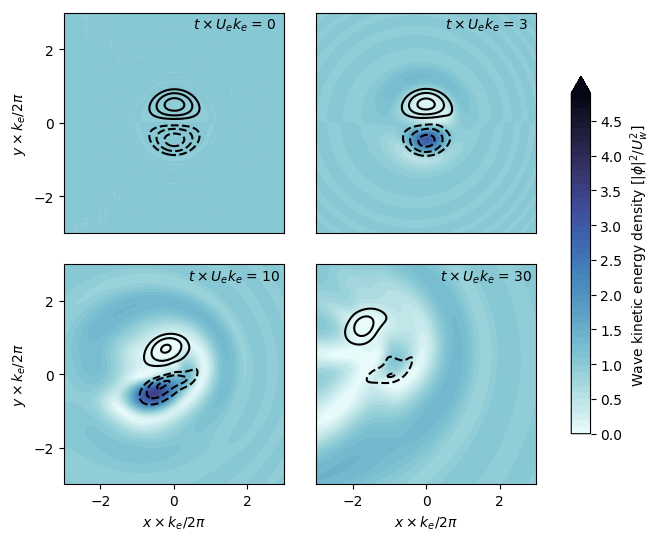
\includegraphics[width=.925\textwidth]{figs/fig1.png}
\caption{Snapshots of the Lamb-Chaplygin dipole solution with parameters presented
          in table \ref{parameters_lamb}.
        Contours depict potential vorticity, $q / (U_e k_e) = [
        -1.5,-0.5,0.5,1.5]$, with dashed lines showing negative values. The upper row shows the wave kinetic energy density $|\phi|^2/2$. The lower row shows the wave buoyancy;
        the buoyancy scale is $B = k_e m U_w f_0 \lambda^2$.
        These plots only show the central $(1/5)^2$
        of the simulation domain.}
\end{figure}

\begin{table}
 \begin{center}
   \caption{Description of parameters of Lamb-Chaplygin simulation.
            The initial condition have Rossby number $Ro = U_e k_e/f_0 \approx
            0.05$, wave dispersivity $\hslash = f_0\lambda^2k_e/U_e
            \approx 1$, and wave amplitude $\alpha = Ro (U_w/Ue)^2 \approx 3.75$.}
   \label{parameters_lamb}
   \begin{tabular}{ l | l | l }
     \hline
      Parameter & Description & Value \\
      \hline
      $R= 2\pi k_e^{-1}$ & Dipole radius & $L_d/15 \approx 84$ km \\
      $U_e$ & Dipole strength & $5\times 10^{-2}$ m s$^{-1}$ \\
      $U_w$ & NIW speed & $5\times 10^{-1}$ m s$^{-1}$ \\
      $N_0$ & Buoyancy frequency & $5 \times 10^{-3}$ s$^{-1}$\\
      $f_0$ & Coriolis frequency & 10$^{-4}$ s$^{-1}$\\
      $2\pi$m$^{-1}$ & NIW vertical wavelength $325$ & m \\
      $\kappa_e$ & QGPV biharmonic diffusivity & $5\times 10^{7}$ m$^4$ s$^{-1}$\\
      $\nu_w$ & NIW biharmonic viscosity & $ 5 \times 10^{7}$ m$^4$ s$^{-1}$\\
      $\mathsf{N}$   & Number of modes &  512  \\
      $L_d$ & Domain size & $2\pi\times 200$ km \\
   \end{tabular}
 \end{center}
\end{table}


As a preamble to our discussion of stimulated generation  in freely-evolving
turbulence, we consider an example in which the initial quasi-geostrophic flow
is the Lamb-Chaplygin dipole---see figure \ref{snaps_lamb}. This dipole is an
exact solution of the Euler equations on an infinite two-dimensional plane where
the vorticity is confined to a circle of radius $R$ \cite[][]{meleshko_vanheijst1994}.
The solution, steady in a frame moving at uniform zonal velocity $U_e$, is
\beq
\label{lambd_q}
  \lap\psi =
     \frac{2 U_e \kappa}{J_0(\kappa R)} \begin{cases}
      J_1(\kappa r)\sin\theta\com & \text{if}
      \qquad r\le R\com\\
      0\com &\text{if} \qquad r\ge R\per
  \end{cases}
\eeq
Above $r^2 = (x-x_c)^2+(y-y_c)^2$ is the radial distance about the dipole's center
$(x_c,y_c)$, $\tan \theta = (y-y_c)/(x-x_c)$, and $J_n$ is the n'th order Bessel function. The matching condition at $r=R$ is that  $J_1(\kappa R)=0$ and the smallest solution is $\kappa R \approx
3.8287$.  If there is no coupling to the wave  $\phi$,  then the dipole \eqref{lambd_q} is a solution of \eqref{macroturb}. The initial wave velocity is  a spatially uniform  near-inertial oscillation with speed $U_w$:
\beq
\label{NIO}
\phi(x,y,t=0) = \tfrac{1 + \ii}{\sqrt{2}}\, U_w\per
\eeq
Further parameters of this dipole solution are summarized in table  \ref{parameters_lamb}.



With the initial condition in \eqref{NIO},  $\qw $  in \eqref{qgpv}  and $\grad \phi$ are both  zero.
The refractive term in the wave equation  \eqref{waves}, however, immediately
imprints itself onto $\phi$ thus creating  non-zero $\grad \phi$ and non-zero
$\qw$. The ensuing wave feedback on the balanced flow results in distortion of
the dipole seen in figure \ref{snaps_lamb}. Once refraction has created gradients
in $\phi$,  the advective term in \eqref{waves} can further distort $\phi$ and increase $\grad \phi$. This scale reduction of $\phi$ is most evident in the wave buoyancy shown in lower
row of figure \ref{snaps_lamb}. Figure \ref{snaps_lamb} also shows the well known focussing  of waves into the negative vortex. But  the wave feedback on the mean flow through $\qw$ then results in distortion and shearing so that the negative vortex loses its integrity  so that the dipole becomes lop-sided and starts to drift. And once the negative vortex  is filamented to small scales it no longer acts as an effective potential well and   the trapping of wave energy  is much less effective than in the initial condition. This phenomenology is also  characteristic of wave-modified two-dimensional turbulence in section \ref{turbulence}.



 To understand the results in
figure \ref{snaps_lamb} and quantify the stimulated generation of wave energy,
we need to understand the  conservation laws of the vertical plane wave model.


\section{Conservation laws of the vertical plane wave model}\label{physics}

XV noted that the vertical plane wave model in \eqref{qgpv} through \eqref{waves} inherits two quadratic conservation laws from the parent  model: if there is no dissipation  then wave action,
\beq
\A \defn  \half |\phi|^2\com
\label{action}
\eeq
and the  energy,
\beq
\E \defn \half |\grad \psi |^2 + \quarter \lambda^2 |\grad \phi|^2  \com
\label{energy}
\eeq
are both separately  conserved.  As explained by  YBJ and XV, the  wave action  in \eqref{action} is also the kinetic energy density of the near-inertial waves. The conserved energy density $\E$ in \eqref{energy} is the sum of the kinetic energy of the balanced flow
\beq
\K\defn \half |\grad\psi|^2\com \label{EKE1}
\eeq
 and  the potential energy of the near-inertial waves,
\beq
\P \defn \half b^2 /N_0^2 = \quarter \lambda^2 |\grad \phi|^2 \per \label{potEnerg}
\eeq
Above, $b\propto \p\phi$ is the wave buoyancy defined in \eqref{buoyancy}. Because $\qw$ is quadratic in $\phi$ the enstrophy  $\la q^2 \ra$ is not a quadratic quantity in the XV model.

XV explain the physical basis of stimulated generation by noting that balanced kinetic energy $\K$ can be converted into wave potential energy $\Pw$ while conserving  the integral of the total energy $\E$  in \eqref{energy}. Indeed, this conversion \textit{must} occur  if $\grad \phi$ is increased by a combination of refraction  and advection in the wave equation \eqref{waves}. In the example shown in  figure \ref{snaps_lamb}, the initial wave field in \eqref{NIO} has infinite spatial scale and therefore there is no  wave potential energy at $t=0$. The subsequent evolution  in figure \ref{snaps_lamb} involves creation of non-zero $\grad \phi$, corresponding to  loss of $\K$  and gain of $\Pw$: this is  stimulated generation of near-inertial waves.

To substantiate this intuition, and diagnose results from our simulation of wave modified two-dimensional turbulence, we  develop the  conservation laws corresponding to \eqref{action} and \eqref{energy} in more detail.



\subsection{The local  action conservation equation }

Multiplying the wave equation  \eqref{waves} by $\phis$ and adding to the complex conjugate we obtain a conservation equation  for action density
\beq
\label{action_density}
\p_t \A + \sJ(\psi,\A) + \diver \Ff =
\half(\phis D_\phi + \phi D_{\phis})
\com
\eeq
where the flux of  \NIW{} action is
\beq
\label{Fw2}
\Ff \defn \tfrac{\ii}{4}\disp\left(\phi\grad\phis-\phis\grad\phi\right) \per
\eeq
The local conservation law  \eqref{action_density} shows how the wave action
$\A$ changes due to divergences of the geostrophic and wave fluxes and dissipation---the second, third, and fourth terms in \eqref{action_density}.



The wave action   flux $\Ff$ is analogous
to the probability current  of quantum mechanics
\citep[e.g., ][pg. 57]{landau_lifshitz2013}. Using the polar representation $\phi = |\phi|\ee^{\ii\Theta}$ the wave action  flux $\Ff$ can also be written as
\beq
\label{Fw2.1}
\Ff =  \A\,  \disp\grad\Theta
\eeq
In \eqref{Fw2.1}
$\disp\grad\Theta$ is the ``generalized group
velocity'' of hydrostatic \NIW s i.e., $\Ff$ is the generalized group velocity times the action density $\A$. We use the term ``generalized'' because  no WKB-type  scale separation is required to obtain the  results above.  The connection to standard internal-wave group velocity is quickly verified by considering a plane near-inertial wave with  $\Theta = kx + ly$ yielding  $f_0\lambda^2\grad\Theta
= {N^2_0}(k,l)/{f_0 m^2}$.

Denoting an average over the domain by $\la \ra$, and assuming that the action  flux divergence $\diver \Ff$ vanishes after integration, we obtain from \eqref{action_density}
\beq
\frac{\dd \la \A \ra}{\dd t} =\epA\ \per
\label{globAct}
\eeq
where $ \epA \defn \la \half(\phis D_\phi + \phi D_{\phis}) \ra$ is the domain average of the dissipative term on the right of \eqref{action_density}.
In the example shown in  Figure \ref{snaps_lamb} the total action $\la \A \ra$ is conserved to within $1$\% over the course of the integration.

The quantum analogy suggests that we should seek an analog of  Ehrenfest's theorem. Thus in  Appendix \ref{AppenB} we develop a local conservation law for $\Ff_t$. The domain average of that result is
\beq
\frac{\dd \la \Ff\ra}{\dd t} =   - \la  \A  \, \grad \half \lap \psi  \ra - \half \disp  \la \ii  \sJ(\phis,\phi) \grad \psi \ra  + \boldsymbol {\varepsilon}_{\Ff}
\label{Ehren}
\eeq
where $\boldsymbol {\varepsilon}_{\Ff}$ is a dissipative term defined in
Appendix \ref{AppenB}. The results in this section are obtained from the wave
equation \eqref{waves} without using the  QGPV equation \eqref{macroturb}. In
other words, \eqref{action_density}-\eqref{Ehren} apply to the YBJ equation with $\ee^{\ii z}$
structure regardless of the balanced flow dynamics.

\subsection{Energy conservation}

The energy conservation law is considerably more complicated than action conservation.  We sequester the details of the local conservation laws to Appendix  \ref{AppenB} and present here the simpler results obtained by domain averaging those local conservation laws.
For the wave potential energy in \eqref{potEnerg} and the balanced kinetic energy in \eqref{EKE1} we find
 \begin{align}
 \frac{\dd \la \P \ra}{\dd t} &= \Gamma_{r} +\Gamma_a + \epP \com \label {ge1} \\
 \frac{\dd  \la \K \ra }{\dd t} &=
 - \Gamma_r - \Gamma_a + \Xi +  \epK \com \label{ge2}
 \end{align}
 where the ``conversion terms'' in \eqref{ge1} and \eqref{ge2}  are
 \begin{align}
 \Gamma_r &\defn f_0^{-1} \Big\la\half\lap\psi \, \diver\Ff \Big\ra\com \label{convr}
 \end{align}
 and
 \beq
  \Gamma_a \defn -\tfrac{\lambda^2}{2}
    \left\la
    \begin{bmatrix}
    \phi_x^\star & \phi_y^\star
    \end{bmatrix}
    \begin{bmatrix}
    -\psi_{xy} & \half(\psi_{xx} - \psi_{yy})\\
    \half(\psi_{xx}-\psi_{yy}) & \psi_{xy}
\end{bmatrix}
  \begin{bmatrix}
    \phi_x \\  \phi_y
    \end{bmatrix}\right\ra\per
    \label{conva}
\eeq
  The dissipative terms, $\epP$,  $\epK$ and $\Xi$  are defined in appendix \ref{AppenB}.  $\Xi$ in \eqref{ge2}  is particularly interesting: dissipation of waves $D_\phi$ produces balanced kinetic energy.
 Summing \eqref{ge1} and \eqref{ge2} the ``conversion'' terms $\Gamma_r$ and $\Gamma_a$  cancel, and we obtain the conservation law for total energy $\la \E \ra=\la \Pw + \K \ra$.

 %% dipole convergence figure %%
 \begin{figure}
 \label{illustration_conversion}
 \centering
 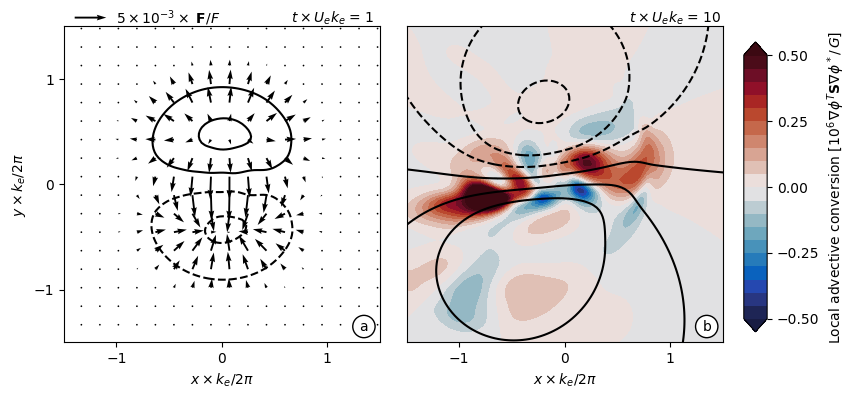
\includegraphics[width=.92\textwidth]{figs/ConversionIllustration.png}
 \caption{Illustration of energy conversion terms in the Lamb-Chaplygin dipole solution
           with parameters presented
           in table \ref{parameters_lamb}. (a) The action density flux $\F$
           overlain on contours of relative vorticity $\lap\psi / (U_e k_e)
           = [-1.5,-0.5,0.5,1.5]$, with dashed lines showing negative values;
           the scale of the action flux is $F = f_0\lambda^2 k_e U_w^2$. (b) The
           local advective conversion
           (i.e., the unaveraged $\Gamma_a$) overlain on contours of streamfunction
           $\psi \times (U_e/k_e)= [-8,-4,-2,0,2,4,8]$.}
 \end{figure}

\begin{figure}
\label{stats_lamb}
\centering
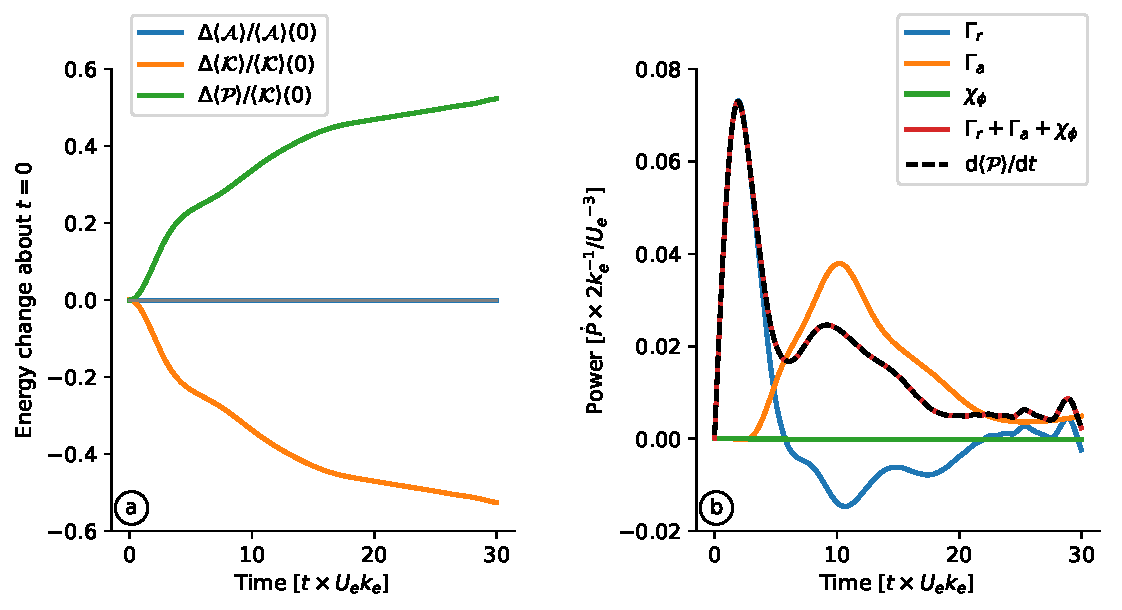
\includegraphics[width=1.\textwidth]{figs/fig2.pdf}
\caption{Diagnostics of the Lamb-Chaplygin dipole solution with parameters presented
          in table \ref{parameters_lamb}. (a) Energy change about initial condition.
        (b) Wave potential energy budget \eqref{ge1}.
        }
\end{figure}



The refractive conversion  $\Gamma_r$   stems from $\ii \phi \lap \psi/2 $  in the wave equation and is easy to
interpret: the convergence of the wave action  flux,
$\nabla\cdot\Ff < 0$, into anticyclones, $\lap\psi<0$, is a source of wave potential energy $\P$.
Figure \ref{illustration_conversion}a shows the convergence of $\F$ into the anti-cyclone
(and divergence from the cyclone) of the dipole solution at $t\times U_e ke = 1$,
which yields the sharp initial increase of $\la P \ra$ discussed below. The unaveraged
Ehrenfest's theorem in \eqref{Ef} illuminates the initial structure of $\Ff$ in
figure \ref{illustration_conversion}. Because $\phi$ is initially uniform, the
initial tendency of $\Ff$ is
\beq
\p_t \Ff \approx -\disp \A\grad \half\lap\psi\per
\eeq
Thus, initially, the wave flux is opposite to the gradient of
relative vorticity as shown in figure \ref{illustration_conversion}.
\textcolor{red}{Check the above expression/conclusion.}


The  advective conversion $\Gamma_a$ in \eqref{ge1} and \eqref{ge2} stems from the term  $J(\psi,\phi)$ in the wave equation \eqref{waves} and is a source of $\la\Pw\ra$ due to straining and deformation of the wave field by the geostrophic flow. The symmetric $2\times 2$ matrix in \eqref{conva} is the strain or deformation tensor of the geostrophic flow. Thus, in analogy with passive scalar gradient amplification \textcolor{cesar}{(Reference?)},   straining also enhances gradients
of the back-rotated near inertial velocity $\phi$, thereby generating wave potential energy, $\la \P \ra$.


\subsection{Energetics of the Lamb-Chaplygin dipole solution}


Figure \ref{stats_lamb} depicts the energetics of the Lamb-Chaplygin dipole
solution discussed above (see also figure \ref{snaps_lamb}). The wave potential
energy increases at the expense of balanced kinetic energy while action is
conserved (Figure \ref{stats_lamb}a). The energy conversion diagnostics show that
the stimulated generation occurs in two stages---see figure \ref{stats_lamb}b. First,
refraction of the initially uniform wave field causes a dramatic concentration
of waves in the anti-cyclone
\citep[cf. ][]{danioux_etal2015}. This initial concentration of the waves in
the anti-cyclone yields a sharp increase in wave potential energy through
$\Gamma_r$. But this sharp initial energy conversion does not last long because
the wave feedback disintegrate the anti-cyclone and dispersion radiates
waves awat from the dipole (Figure \ref{snaps_lamb}). Thus $\Gamma_r$ decreases
sharply, eventually reversing sign at $t\times U_e k_e\approx 8$.

The second stage of stimulated generation in the dipole solution starts when
refraction creates dipole-scale waves. Advection by the balanced flow
strains the waves, further reducing their lateral scale (Figure
\ref{stats_lamb}b). The ensuing advective conversion, $\Gamma_a$, starts
at $t\times U_e k_e \approx 4$. Straining by the balanced flow sustains this
advective generation of wave potential energy. Most of the energy eventually
escapes the straining regions through dispersion and the conversion nearly halts at
$t\times U_e k_e = 30$.
The time-integrated $\Gamma_a$ accounts for $\approx 78\%$ of the
wave potential energy generation; table \eqref{table1} contains the details
of the energy budgets of this dipole solution.

% adds table 1, which is an output of a python script
% This is preferable, on reproducibility grounds, than adding values manually.
%\begin{table}
\begin{center}
\caption{The time-integrated budget of wave potential energy and quasigeostrophic                kinetic energy of the Lamb-Chaplygin dipole expirement. \label{table1}}
\begin{tabular}{cccc}
$\dot{P}_w$ budget & Rel. contribution ($\int\dot{P}_w \dd t/\Delta P_w dt$) & $\dot{K}_e$ budget & Rel. contribution ($\int\dot{K}_e \dd t/\Delta K_e$) \\
$\Gamma_r$ & 1.2 & -$\Gamma_r$ & -0.551 \\
$\Gamma_a$ & 2.148 & -$\Gamma_a$ & -0.987 \\
$-$ & $-$ & $\Xi_r$ & 0.855 \\
$-$ & $-$ & $\Xi_a$ & 0.022 \\
$\chi_\phi$ & -2.348 & $\epsilon_\psi$ & -0.338 \\
Res. & 0.0 & Res. & 0.0 \\
\end{tabular}
\end{center}
\end{table}

\begin{table}
\begin{center}
    \caption{The time-integrated budget of wave potential energy and quasig-eostrophic                kinetic energy of the Lamb-Chaplygin dipole solutions with parameters provided in table \ref{parameters_lamb}. The energy budgets close within $10^{-6}\,\%$.\label{table1}}
\begin{tabular}{c|c|c|c}
\hline
$\dot{P}_w$ budget & Fractional size ($\int\dot{P}_w \dd t/\Delta P_w $) & $\dot{K}_e$ budget  & Fractional size ($\int\dot{K}_e \dd t/\Delta K_e$)\\
\hline
$\Gamma_r$ & 0.228 & -$\Gamma_r$ & -0.227 \\
$\Gamma_a$ & 0.778 & -$\Gamma_a$ & -0.774 \\
$-$ & $-$ & $\Xi_r$ & 0.004 \\
$-$ & $-$ & $\Xi_a$ & 0.0 \\
$\chi_\phi$ & -0.006 & $\epsilon_\psi$ & -0.003 \\
Res. & 0.0 & Res. & 0.0 \\
\end{tabular}
\end{center}
\end{table}

%
% The uncoupled \cite{young_benjelloul1997} equation with barotropic geostrophic flow
% and single propagating vertical mode near-inertial
% also satisfies the potential energy equation \eqref{Pw}. But
% \cite{young_benjelloul1997} and subsequent studies overlooked the wave potential
% energy power integral, \eqref{Pw}, or its generalization to baroclinic quasi-geostrophic flow.
% Of course, the standard Young
% \& Ben Jelloul wave equation is uncoupled from the quasi-geostrophic potential
% vorticity equation, hence an increase in wave potential energy is not matched by a
% decrease in geostrophic kinetic energy.

%\subsection{Averaged equations and loss of coherence}
%The spatially-averaged (coherent) wave amplitude satisfies
%\beq
%\label{phi_ave}
%\frac{\dd}{\dd t}\la \phi \ra + \ii \left\la\half\phi\lap\psi \right\ra =
%D_{\la\phi\ra}\per
%\eeq
%Introducing the decomposition $\phi = \la\phi\ra+\phi'$, we have
%\beq
%\half\la|\phi|^2\ra
%= \underbrace{\half|\la\phi\ra|^2}_{\defn K^c_w} +
%\underbrace{\half\la|\phi'|^2\ra}_{\defn K^i_w}\com
%\eeq
%Thus, the kinetic energy of horizontally incoherent, $\phi'$, and coherent,
% $\la\phi\ra$, waves satisfy
%\beq
%\label{Kiw}
%\dot{K}_w^i = \Pi + \varepsilon_{\la\phi\ra}\com
%\eeq
%and
%\beq
%\label{Kcw}
%\dot{K}_w^c = -\Pi + \varepsilon_{\phi'}\com
%\eeq
%with the kinetic energy transfer
%\beq
%\label{Pi}
%\Pi = \tfrac{\ii}{2}\left[\la\half\phi\lap\psi\ra\la\phis\ra -
%\la\half\phis\lap\psi\ra\la\phi\ra\right]\com
%\eeq
%which measures the loss of lateral coherence of the wave field. Also in \eqref{Kiw}
%and \eqref{Kcw}, $\varepsilon_{\la\phi\ra}$ and $\varepsilon_{\phi'}$ are the dissipation
%of kinetic energy of incoherent and coherent waves, respectively.
%
% \subsection{Relevant parameters}
% Consider the scaling
% \beq\label{scaling}
% \psi \sim U_e k_e^{-1} \com\qquad \text{and} \qquad \phi \sim U_w\com
% \eeq
% with characteristic QG and NIW velocity scales $U_e$ and $U_w$, and the
% characteristic horizontal length scale $k_e^{-1}$ and time scale $(U_e k_e)^{-1}$.
% Using \eqref{scaling} in \eqref{macroturb}-\eqref{waves}
% reveals that there are two dynamically relevant parameters of the QG-NIW problem
% described by \eqref{macroturb}-\eqref{waves}. First, the `wave amplitude'
% \beq
% \label{alpha}
% \alpha \defn \underbrace{\frac{U_e k_e}{f_0}}_{\defn Ro} \times
% {\left(\frac{U_w}{U_e}\right)^2}\com
% \eeq
% measures the strength of the waves compared to the geostrophic flow and scales
% the contribution of the wave terms in the potential vorticity \eqref{qgpv}.
% Second, the `wave dispersivity,'
% \beq
% \label{hslash}
% \hslash \defn f_0 \lambda^2 \times \frac{k_e}{U_e}\com
% \eeq
% scales the importance of linear dispersion, which extenuates the unsmoothing
% effects of advection and refraction.

\subsection{Summary}
% The following initial value problem that idealizes the oceanographic post-storm scenario
% illuminates the physics of stimulated generation. Stormy winds impart momentum
% into the ocean, thereby generating near-inertial oscillations with a lateral
% decorrelation scale larger than the mesoscale eddies. The coupled model
% \eqref{macroturb}--\eqref{waves} describes the post-storm evolution
% of this initially coherent inertial oscillation
%  \citep{xie_vanneste2015,wagner_young2016}. Geostrophic refraction
% concentrates the waves in anticyclones. The eddy-scale gradients of $\phi$ then support
% geostrophic advection. Advection and refraction reduce the lateral coherence
% of the waves---and wave dispersion counteracts this unsmoothing effect.

The explicit expression for energy conversion on the right of \eqref{ge1} and \eqref{ge2} clarify the mechanism of stimulated generation of an initially uniform \NIW. First, refraction causes a convergence of wave
kinetic energy density in anti-cyclones. Then, advection strains the waves, reducing their lateral scale. Both
processes amplify the lateral gradients of wave amplitude, thereby generating wave potential energy $\Pw$ at the expense of balanced kinetic energy $\K$.

In the remainder of this paper, we describe and quantify the stimulated generation of an initially uniform \NIW interacting with decaying turbulence, which is an idealization of the oceanographic post-storm scenario.

% \section{An idealized solution: the Lamb-Chaplygin dipole}\label{dipole}
%
% \subsection{Solution for $\hslash \approx 1$ and $\alpha \approx 3.75$}
% We solve the coupled model \eqref{macroturb}-\eqref{waves} subject to the
% initial conditions \eqref{lambd_q} and \eqref{NIO} and the parameters inspired
% by the Ocean Storms Experiment. We integrate the solutions numerically
%  for $30$ eddy-turnover time units,
% $30\times (U_e k_e)^{-1}\approx 90$ days, on a
% doubly periodic domain using standard Fourier pseudo-spectral methods (detail in appendix B).
% Dipole images, artifacts of periodization,
% cause a small zonal drift of the dipole. To render this drift negligible, we
% choose a domain size much larger than the dipole's radius, $R/L \approx 0.06$.
% Table B.1 provides a full description of solution parameters.
%
% Because the initial wave velocity is laterally uniform, refraction dominates
% the initial evolution of the solution.
% Indeed, the solution presents a dramatic wave concentration
% in the anticyclone and wave expulsion from the cyclone in the first couple of
% eddy turnover time units, $(U_e k_e)^{-1}$. After $5 \times (U_e k_e)^{-1}$, there
% is a threefold modulation of the wave kinetic energy density on eddy scales
% (Figure \ref{snaps_lamb}). The  correlation coefficient
% \beq
% \label{corr_r}
% r \defn \frac{\left\la |\phi'|^2\,\lap\psi\right\ra}{
% \left\la |\phi'|^4\right\ra^{1/2} \left\la (\lap \psi)^2\right\ra^{1/2}}\com
% \eeq
% quantifies the wave concentration in regions positive or negative vorticity;
% negative correlation, $r<0$, indicates wave concentration in anticyclones
% \citep{danioux_etal2015}. Starting form the uniform wave initial condition,
% vorticity and incoherent wave kinetic energy density
% quickly become negatively correlated ($r=-0.75$ at $t\times U_e k_e$ = 2;
% Figure \ref{stats_lamb}d). This initial wave focusing in anticyclones is associated
% with a rapid increase in incoherent wave kinetic energy (Figure \ref{stats_lamb}c)
% and a rapid increase of wave potential energy (Figure \ref{stats_lamb}b). The gain of
% wave potential energy, ininitially dominated by the conversion due to refraction,
% $\Gamma_r$,
%  occurs at the expenses of geostrophic kinetic energy
% (Figure \ref{stats_lamb}a):
% the dipole's kinetic energy decays by about 20$\%$ in two eddy-turnover time units.
% The strong wave concentration in the negative vorticity region, and the accompanying
% geostrophic energy loss, weakens the anticyclone.  This asymmetry in wave concentration
% tilts the dipole and the vortex self-induced zonal velocity no longer matches the
% downstream uniform flow: the dipole starts to drift upstream at $t\times U_e
% k_e \approx 5$.
%
% % Now comment on the advection conversion (and wave dispersion)...
% The eddy-scale gradients in wave velocity, which are created by refraction,
%  allow for the other mechanisms in the wave equation \eqref{waves} to become
%  important. Linear dispersion radiates waves from the dipole, with horizontal
% scales comparable to $k_e^{-1}$. And geostrophic advection starts to enhance
%  the refraction-created gradients. As a consequence of these two processes becoming
%  important, the correlation $r$ decreases.
%
% The advective conversion, $\Gamma_a$, kicks
% off at $t\times U_e k_e \approx 4$ (Figure \ref{stats_lamb}b), and takes over
% the $\Gamma$ in few eddy-turnover time units. Contemporarily, the wave-induced
% quasi-geostrophic flow strains the anticyclone, which develops a filamentary structure.
% Because most of the advective energy conversion occurs in the anticyclone, the
% negative correlation $r$ decreases further, and becomes positive at
% $t\times U_e k_e \approx 7$. At this point, $\Gamma_r$ becomes weakly negative
% (i.e., from waves to geostrophic flow), though the total conversion, $\Gamma_r
% + \Gamma_a$, remains positive thanks to a strong positive advective conversion.
% The energy conversion nearly halts at $t\times U_e k_e \approx 20$.
%
% Because the advective conversion, $\Gamma_a$, remains positive for the duration
% of the simulation, $\Gamma_a$ accounts for the bulk conversion of energy from
% geostrophic flow to waves. Indeed, the time-integrated $\Gamma_a$ accounts for $77.5\%$
% of total geostrophic kinetic energy change (Table \ref{table1}); the time-integrated
% refraction conversion, $\Gamma_r$, represents $22.7\%$ of the geostrophic kinetic
% energy changes. And direct dissipation and wave-dissipation source
% (Appendix B) account for the residual changes ($<1\%$).



\section{Decaying macroturbulence modified by \NIW s}\label{turbulence}

To study the energy exchange between near-inertial waves and quasi-geostrophic flow
in an oceanographic turbulent regime, we consider a barotropic flow that emerges from
random initial conditions integrated for 20 eddy turnover time units.
In other words, we first integrate the initial condition
\beq
\label{psi_init}
\psi \big(x,y, t \times U_e k_e = -20\big) = \sum_{k,l} |\hat{\psi}|\cos\left(k x + l y +
\chi_{k,l}\right)
\eeq
with waveless quasi-geostrophic dynamics before introducing waves at $t\times U_e k_e = 0$.
Above, $\chi_{k,l}$ is a random phase uniformly distributed on $[0, 2\pi)$,
 and $|\hat\psi|$ is the streamfunction isotropic spectrum
\beq
\label{psih_mag}
|\hat{\psi}| = C \times \big\{|k|\,[1 + (|k|/k_e)^4]\big\}^{-1/2}\com
\eeq
with the wavenumber magnitude $|k|^2 = k^2 + l^2$. The prescribed initial energy
$U_e^2/2$ determines the constant C:
\beq
\label{ke_init}
\sum_{k,l} \underbrace{|k|^2 |\hat{\psi}|^2}_{\defn \cK_e} = \tfrac{1}{2}U_e^2\per
\eeq
The kinetic energy spectrum, $\cK_e$, peaks at the energy-containing scale $k_e^{-1}$.
At scales larger than $k_e^{-1}$, $\cK_e$ has a linear dependence on $|k|$,
whereas $\cK_e$ decays as $|k|^{-3}$ at scales smaller than $k_e^{-1}$. This red spectrum
ensures insignificant energy loss by small-scale dissipation in \eqref{macroturb}.

 The evolution of a random initial condition constrained by the quasi-inviscid
 quasi-geostrophic dynamics \eqref{macroturb} has been well studied, beginning
with \cite{fornberg1977}.
 Stirring of vorticity, $\lap \psi$, by the flow, $\psi$, transfers enstrophy towards
 small scales; energy flows to large
 scales. Most of enstrophy is dissipated within few eddy turnover time units, whereas
 kinetic energy is nearly conserved. Vorticity concentrates into localized
 structures: after 20 eddy turnover time units, the vorticity is well-organized
 into a sea of coherent vortices that form via like-sign vortex merging
 \citep[e.g., ][]{mcwilliams1984}.

 We add a uniform near-inertial oscillation \eqref{NIO} to the mature
 barotropic turbulence at $t \times U_e k_e = 0$. For all parameters considered
 in the remainder of the paper, there are no qualitative long-term differences
 between the solutions described below and results from introducing the waves
 at $t\times U_e k_e = -20$.

 \subsection{Relevant parameters}
Using the scaling
 \begin{align}\label{scaling}
    \text{length}    \sim  k_e^{^{-1}}\com\qquad
    \text{time}    \sim (U_e k_e)^{^1}\com\qquad
    \psi \sim U_e k_e^{-1} \com
    \text{and}\qquad\phi \sim U_w\com
 \end{align}
 shows that there are two dynamically relevant parameters of this decaying
 two-dimensional turbulence modified by \NIW s. First, the `wave amplitude'
 \beq
 \label{alpha}
 \alpha \defn \underbrace{\frac{U_e k_e}{f_0}}_{\defn Ro} \times
 {\left(\frac{U_w}{U_e}\right)^2}\com
 \eeq
 measures the strength of the waves compared to the geostrophic flow and scales
 the contribution of the wave terms in the potential vorticity \eqref{qgpv}.
 \textcolor{cesar}{Shall we remark in passing that $\alpha\sim\mathcal{O}(1)$ is the asymptotic
 regime of validity of XV the model?}
 Second, the `wave dispersivity,'
 \beq
 \label{hslash}
 \hslash \defn \disp \times \frac{k_e}{U_e}\com
 \eeq
 scales the importance of linear dispersion, which extenuates the unsmoothing
 effects of advection and refraction.

 \begin{table}
  \begin{center}
    \caption{Description of parameters of the macroturbulence simulations.
             The initial condition have Rossby number $Ro = U_e k_e/f_0 \approx
             0.05$, wave dispersivity $\hslash = f_0\lambda^2k_e/U_e
             \approx 0.5-2$, and wave amplitude $\alpha = Ro (U_w/Ue)^2 \approx 0.2$.}
    \label{parameters_turb}
    \begin{tabular}{ l | l | l }
      \hline
       Parameter & Description & Value \\
       \hline
       $R= 2\pi k_e^{-1}$ & Energy-containing scale & $L_d/10 \approx 125$ km \\
       $U_e$ & Eddy velocity & $5\times 10^{-2}$ m s$^{-1}$ \\
       $U_w$ & NIW speed & $1 \times 10^{-1}$ m s$^{-1}$ \\
       $N_0$ & Buoyancy frequency & $5 \times 10^{-3}$ s$^{-1}$\\
       $f_0$ & Colioris frequency & 10$^{-4}$ s$^{-1}$\\
       $2\pi$m$^{-1}$ & NIW vertical wavelength $280-560$ & m \\
       $\kappa_e$ & QGPV biharmonic diffusivity & $5\times 10^{6}$ m$^4$ s$^{-1}$\\
       $\nu_w$ & NIW biharmonic viscosity & $ 5 \times 10^{6}$ m$^4$ s$^{-1}$\\
       $\mathsf{N}$   & Number of modes &  1024  \\
       $L_d$ & Domain size & $2\pi\times 200$ km \\
    \end{tabular}
  \end{center}
 \end{table}

 \begin{figure}
 \label{snaps_turb}
 \centering
 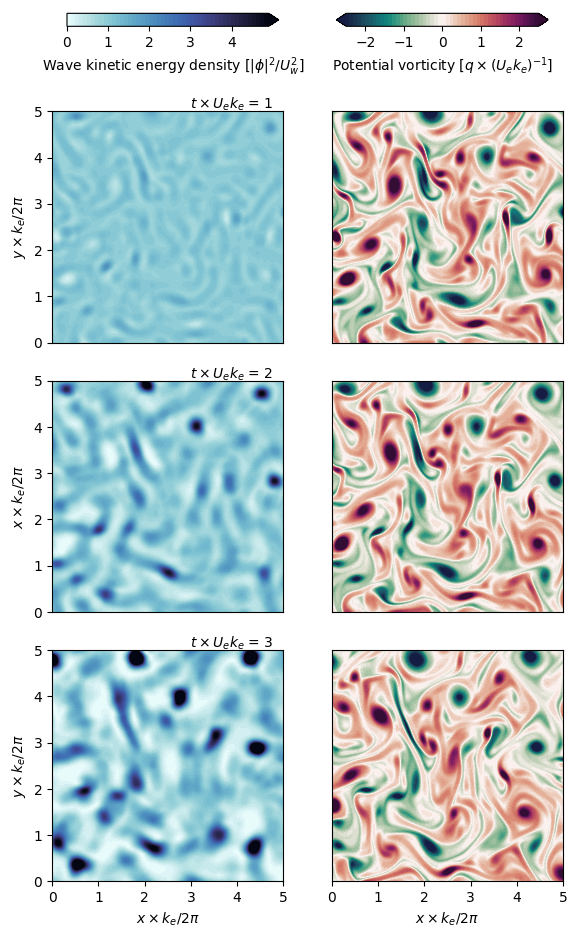
\includegraphics[width=1.\textwidth]{figs/fig3.png}
 \caption{Snapshots of the decaying turbulence solution with parameters shown in
          table \ref{parameters_turb}. Upper panels: quasi-geostrophic potential vorticity
          (QGPV). Middle panels: wave kinetic energy (KE) density.
         Bottom panels: wave buoyancy, whose scale is $B = k_e m U_w f_0 \lambda^2$.
        These plots only show the bottom-left
        $(1/2)^2$ of the simulation domain.}
 \end{figure}

 \begin{figure}
 \label{stats_turb}
 \centering
 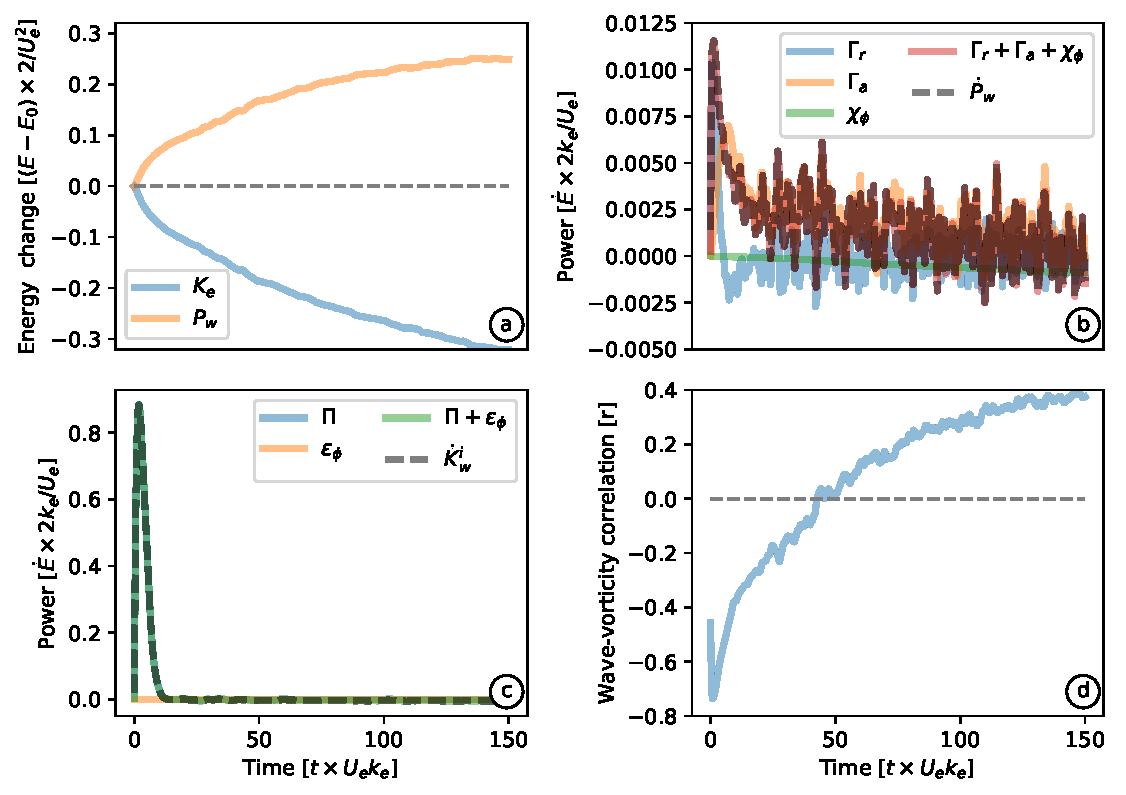
\includegraphics[width=1.\textwidth]{figs/fig4.pdf}
 \caption{Diagnostics of the macroturbulence solution with parameters presented
           in table \ref{parameters_turb}. (a) Energy change about initial condition.
         (b) Wave potential energy budget \eqref{Pw}.
         }
 \end{figure}

 \begin{figure}
 \label{pv-terms_turb}
 \centering
 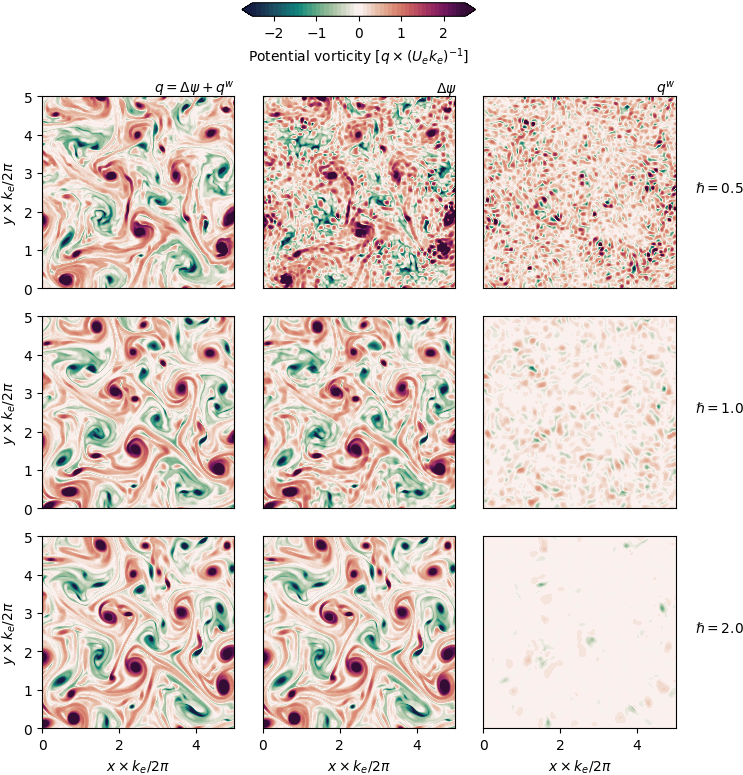
\includegraphics[width=1.\textwidth]{figs/fig5.png}
 \caption{Snapshots of quasi-geostrophic potential vorticity and its
          decomposition into relative vorticity $\lap\psi$, and wave
          potential vorticity $q^w$. The snapshots were taken at $t\times U_e k_e =25$.
         }
 \end{figure}


 % adds table 2, which is an output of a python script
 % This is preferable, on reproducibility grounds, than adding values manually.
 %\begin{table}
\begin{center}
\caption{The time-integrated budget of wave potential energy and quasigeostrophic                kinetic energy of the decaying turbulence dipole expirement. \label{table2}}
\begin{tabular}{cccc}
$\dot{P}_w$ budget & Rel. contribution ($\int\dot{P}_w \dd t/\Delta P_w dt$) & $\dot{K}_e$ budget & Rel. contribution ($\int\dot{K}_e \dd t/\Delta K_e$) \\
$\Gamma_r$ & 0.002 & -$\Gamma_r$ & -0.002 \\
$\Gamma_a$ & 1.129 & -$\Gamma_a$ & -0.955 \\
$-$ & $-$ & $\Xi_r$ & 0.035 \\
$-$ & $-$ & $\Xi_a$ & -0.001 \\
$\chi_\phi$ & -0.131 & $\epsilon_\psi$ & -0.078 \\
Res. & 0.0 & Res. & -0.0 \\
\end{tabular}
\end{center}
\end{table}





 \begin{table}
 \begin{center}
     \caption{The time-integrated budget of wave potential energy and quasi-geostrophic
              kinetic energy of the reference macroturbulence solution with
              parameters in \ref{parameters_turb}. The energy budgets close
              within $10^{-1}\,\%$.\label{table2}}
 \begin{tabular}{c|c|c|c}
 \hline
 $\dot{P}_w$ budget & Fractional size ($\int\dot{P}_w \dd t/\Delta P_w $) & $\dot{K}_e$ budget  & Fractional size ($\int\dot{K}_e \dd t/\Delta K_e$)\\
 \hline
 $\Gamma_r$ & 0.117 & -$\Gamma_r$ & -0.108 \\
 $\Gamma_a$ & 0.907 & -$\Gamma_a$ & -0.839 \\
 $-$ & $-$ & $\Xi_r$ & 0.009 \\
 $-$ & $-$ & $\Xi_a$ & 0.003 \\
 $\chi_\phi$ & -0.026 & $\epsilon_\psi$ & -0.062 \\
 Res. & 0.003 & Res. & 0.003 \\
 \end{tabular}
 \end{center}
 \end{table}

 % \begin{figure}
 % \label{bulk_stats_turb_various}
 % \centering
 % 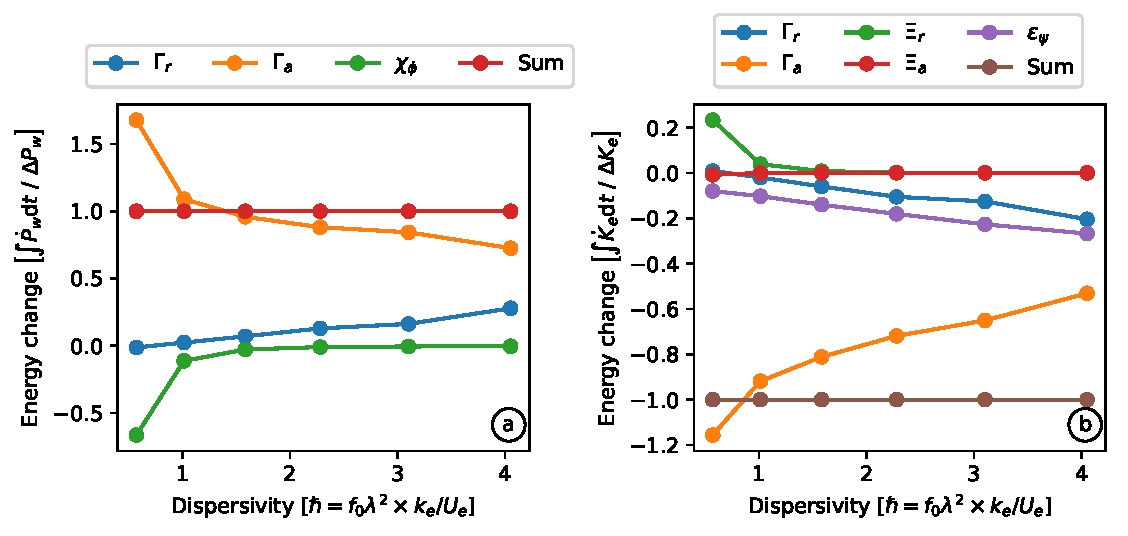
\includegraphics[width=1.\textwidth]{figs/fig7.pdf}
 % \caption{Energy budgets of the decaying turbulence solution $\alpha \approx 1$ and
 %         different dispersivities, $\hslash$. (a) Wave potential energy budget.
 %         (b) Geostrophic kinetic energy budget.
 %         }
 % \end{figure}


% \subsection{Parameters for strong mid-latitude macroturbulence}
%
% Consider strong mid-latitude macroturbulence, such as the Gulf Stream or Kuroshio
% Extension. The choice of parameters, $U_e = 0.1$ m s$^{-1}$,
% $f_0 = 1 \times 10^{-4}$ s$^{-1}$, $2\pi k_e^{-1} = 125$ km
% gives a Rossby number $Ro \approx  0.05$. For reference, the eddy-turnover scale
% is $(U_e k_e)^{-1}\approx 5.8\,\,\text{days}$. Strong near-inertial velocity
% imparted by atmospheric storms, $U_w \sim \sqrt{2} U_e$, implies a wave amplitude
% \beq
%   \alpha \approx 0.1\per
% \eeq
% A near-inertial vertical wavelength of $\lambda_z = 2\pi/m = 300$ m \citep[e.g., ][]{alford_etal2016}
% on a strongly stratified upper ocean, $N_0/f_0 = 100$, yields a dispersivity
% \beq
%   \hslash \approx 1.0 \per
% \eeq

\subsection{Solution with $\hslash = 1$ and $\alpha = 0.1$}

% General remarks about the flow evolution
Figure \ref{snaps_turb} show snapshots of a solution with
$\hslash = 1$ and $\alpha = 0.1$ and further parameters in table \ref{parameters_turb}.
This turbulence solution shares qualitative aspects of the Lamb-Chaplygin solution.
Starting from a uniform wave field, refraction quickly concentrates the waves into
anti-cyclones. By
$t\times U_e k_e \approx 1$ there is a two-fold modulation of the wave kinetic
energy density on eddy scales. with significant focusing of waves in anti-cyclones
(compare middle and upper panels of figure \ref{snaps_turb}).

The eddy-scale gradients of wave velocity support geostrophic advection and
wave dispersion. Dispersion radiates waves from the vortices; advection enhances
the gradients of the wave back-rotated velocity (see lower panels of figure \ref{snaps_turb},
which depict wave buoyancy). By $t\times U_e k_e \approx 10$ there is a five-fold
modulation of the wave kinetic energy density and the wave buoyancy has been
amplified by a factor of two. The potential vorticity evolves similarly to the
two-dimensional problem: like-sign vortices merge into bigger vortices. The big
vortices keep straining the waves, generating finer scales.

% The energetics
The initial refractive effects cause an initial sharp generation of wave potential
energy, which occur at the expense of balanced kinetic energy---see
figure \ref{stats_turb}a. As in the Lamb-Chaplygin solution, the positive refractive
conversion, $\Gamma_r > 0$, is ephemeral: its peaks at $t\times U_e k_e \approx 2$ and decays
sharps, eventually changing sign at $t\times U_e k_e \approx 5$ (figure \ref{stats_turb}a).
But a significant positive advective conversion, $\Gamma_a> 0$, sustains the
wave stimulated generation. From $t\times U_e k_e \gtrsim 4$ the wave potential energy
increases approximately linearly.

After 25 eddy-turnover time units, the balanced kinetic energy decays by about
$14 \%$ of the initial condition. Most of this loss of balanced energy is accounted
by the generation of wave potential energy. As in the Lamb-Chaplygin solution,
advective conversion accounts for most of the energy change, representing about
84$\%$ of the balanced energy changes. Further details of the energy budget are
presented in table \ref{table2}.

% Now discuss the main features
The solution above depicts interesting characteristics of the stimulated generation
of an initially uniform near-inertial wave. First, the role of refraction appears
to be catalytic in that it generates the eddy-scale gradients in the wave field
that are then enhanced by geostrophic straining, which accounts for the bulk
energy transfer. Second, the wave potential energy growth is very slow in comparison
with exponential prediction from the passive scalar problem. This slow energy
growth suggests that wave dispersion play an important role in slowing the
straining. To investigate whether these characteristics are general we consider
solution with varying vertical wavelengths and therefore different dispersivities.

% Besides the energy extraction from the decaying turbulence flow, the waves
% also cause larger direct dissipation of geostrophic kinetic energy compared with
% a waveless QG solution with the same parameters (Appendix B). In the waveless solution
% the dissipation, $\varepsilon_\psi$, is about $2\%$, most of which occurs at
% $t\times U_e k_e < 20$. The direct dissipation of geostrophic kinetic energy is
% a consequence of the small-scale diffusion introduced in the potential vorticity equation
% \eqref{macroturb}. Hence, the stronger
% dissipation in the coupled model is due to finer scaler developed in the relative
% and potential vorticities, $\lap\psi$ and $q$. Indeed,
% $\lap\psi$ has more texture than than waveless vorticity
% (compare figure \ref{pv-terms_turb} with figure C1),
% particularly outside the core of the vortices (Figure \eqref{pv-terms_turb}b).
% The wave terms of the potential vorticity  are dominated by small scales and
% smaller than $\lap\psi$ (Figure \eqref{pv-terms_turb}c-d). Interestingly, much
% of the roughness in $\lap\psi$ is canceled by the small-scale structures in the
% wave potential vorticity, yielding a
% smoother---but rougher than waveless QG---potential vorticity
%  (compare figures \ref{snaps_turb} with figure C2).

\subsection{Varying dispersivity}
\begin{figure}
\label{stats_turb_various}
\centering
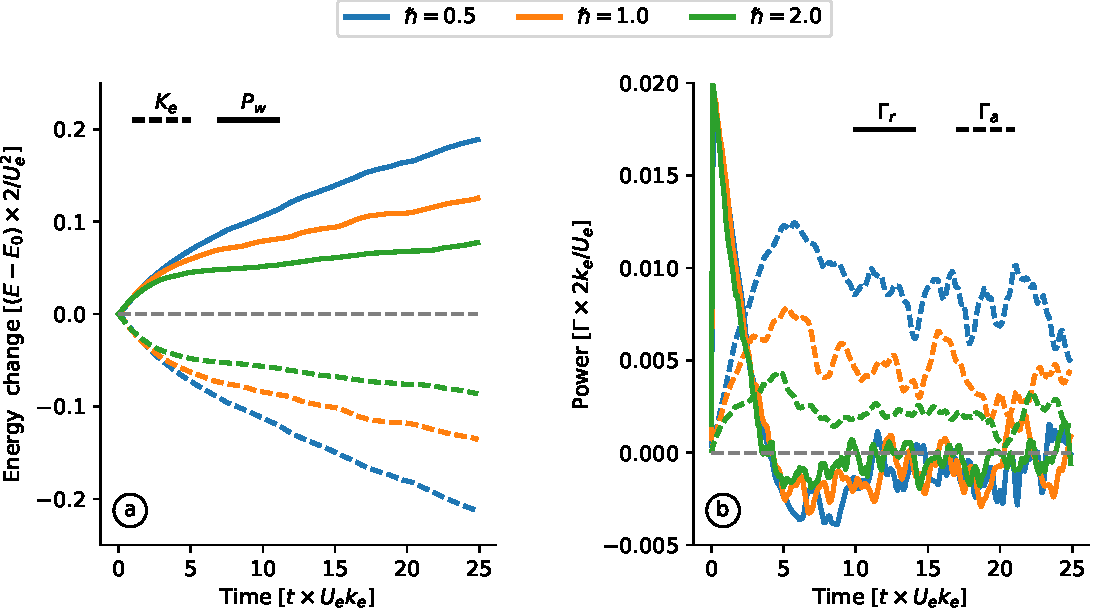
\includegraphics[width=1.\textwidth]{figs/fig6.pdf}
\caption{The energetics of macroturbulence solutions with different
         dispersivities. (a) Energy change about the initial condition.
         (b) The energy conversion terms in \eqref{ge1}.
        }
\end{figure}

\begin{figure}
\label{spectra_turb_various}
\centering
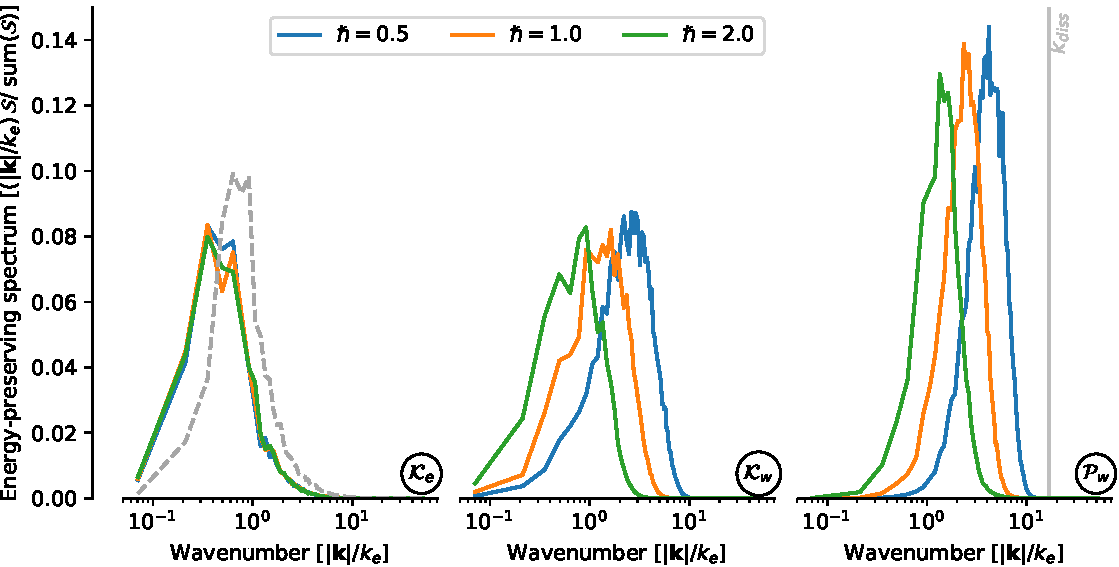
\includegraphics[width=1.\textwidth]{figs/FigSpectraVarious.pdf}
\caption{Energy-preserving spectra of macroturbulence solutions with different
         dispersivities. Different panels show spectra at of balanced kinetic energy
          $\mathcal{K}_e$, wave kinetic energy $\mathcal{K}_w$, and wave potential
          energy $\mathcal{P}_w$. All solid lines correspond to spectra at
          $t\times U_e k_e = 25$ and the dashed line in $\mathcal{K}_e$ depicts
          the balanced kinetic energy spectrum at $t\times U_e k_e = 0$.
        }
\end{figure}

Figure \ref{stats_turb_various}
shows potential vorticity snapshots of a set of solutions with varying the vertical wavelength
$2\pi\,m^{-1}$ from 280 to 560 m, yielding dispersivities ranging from 0.5 to 2.
(All other parameters are fixed.) The potential vorticity $q$ shows more small-scale
filamentation with decreasing dispersivity, but it is otherwise similar across
the solutions. The partition into relative vorticity $\lap\psi$ and wave potential
vorticity $\qw$, however, depends significantly on dispersivity. In particular,
$\qw$ develops smaller scales and larger amplitudes with decreasing dispersivity.
Interestingly, there is strong cancellation of small-scale features in $\qw$
and $\lap\psi$, yielding a smooth $q$ even in the weak dispersion solution.

The initial evolution of the uniform wave field is similar across dispersivities,
with refraction generating eddy-scale gradients of the waves---see figure \ref{stats_turb_various}.
Refraction thus yields an initial increase of wave potential energy and decrease
of balanced kinetic energy, which is almost independent of dispersivity. Once the
eddy-scales are created, advection strains the waves further generating wave
potential energy at the expense of balanced kinetic energy. It is in this stage
that the dependence on dispersivity is pronounced. Weakly dispersive waves are
strained further than strong dispersive waves. Thus the advective conversion becomes
stronger with decreasing dispersivity (figure \ref{stats_turb_various}b).

The balanced dynamics evolves similarly to the waveless decaying macroturbulence.
That is, there is a transfer of balanced energy towards larger scales with like-sign
vortices mergers (figure \ref{spectra_turb_various}a). The main difference is that
balanced kinetic energy is not conserved; kinetic energy is constantly transformed
in wave potential energy via stimulated generation. The stimulated generation process
is associated with a forward transfer of wave action from the infinite horizontal
scales to eddy scales figure \ref{spectra_turb_various}b). The wave potential
energy density develops scales smaller than eddy scales (figure
\ref{spectra_turb_various}c).

\begin{figure}
\label{correlation_skewness}
\centering
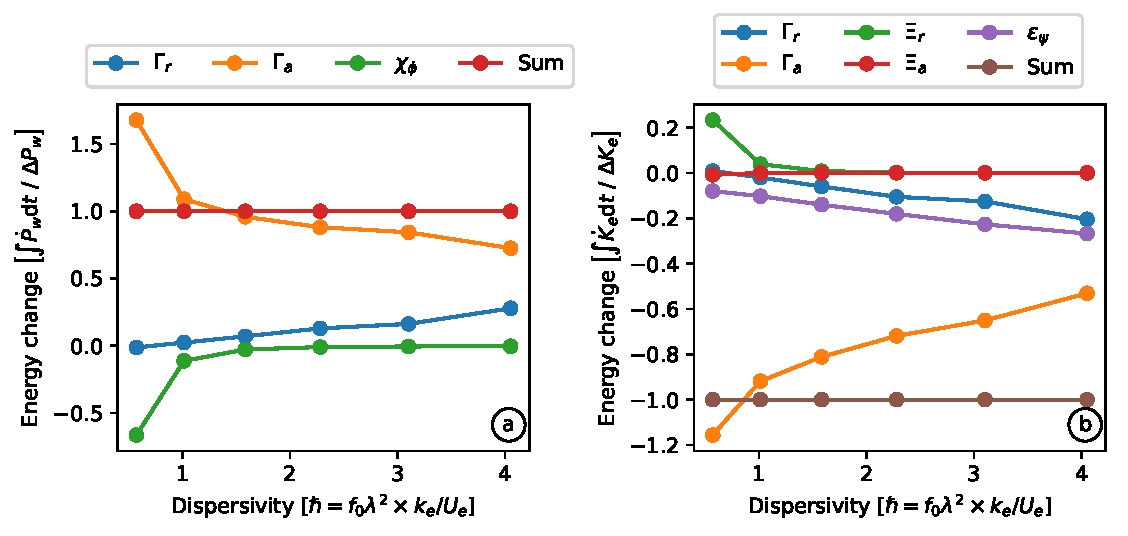
\includegraphics[width=1.\textwidth]{figs/fig7.pdf}
\caption{Diagnostics of macroturbulence solutions with different
         dispersivities. (a) The correlation between relative vorticity and
         wave kinetic energy. (b) The skewness of relative vorticity.
        }
\end{figure}


\section{Discussion}\label{discussion}
The explicit expression for the energy conversion in \eqref{ge1} illuminates the
physics of stimulated generation: both convergence of wave kinetic energy density
in anticyclones and geostrophic straining are sources of wave potential
energy and sinks of geostrophic kinetic energy. But this energy description
of stimulated generation disguises the role of wave dispersion---waves can
propagate out of the vorticity or straining regions, thereby reducing the
correlations of the energy conversion in \eqref{ge1}.

% Wave scaping
Indeed, wave dispersion is the only mechanism that upsets stimulated generation
in the quasi-inviscid solutions described in this paper. In all solutions, after
an initial conversion due to refraction,
geostrophic straining accounts for most of the energy conversion. But even in the
weak dispersion solution, the waves not behave as a passive scalar. This is
because geostrophic advection can only strain the near-inertial wave field so much.
The near-inertial generalized group velocity is $f_0\lambda^2\grad\Theta$
(cf. section \ref{physics}), where $\Theta$ is the phase of the near-inertial
back-rotated velocity: $\phi = |\phi|\ee^{\ii\Theta}$. With fixed dispersivity,
$f_0\lambda^2$, the very geostrophic straining, enhances the gradients $\grad\Theta$,
thereby increasing the near-inertial group velocity: the waves scape the straining
region. Thus, the mechanism of wave capture \citep{buhler_mcintyre2005} does not
occur in the solutions described above.

 The geostrophic straining accounts for the bulk energy transfers in the examples
with initially large-scale \NIW s, which represent a sink of
$5-50\%$ of the initial geostrophic kinetic energy. But refraction plays a fundamental role
in these solutions with uniform (laterally coherent) initial wave velocity.
 This initial condition idealizes the
generation of upper-ocean inertial oscillations by storms
\citep[e.g., ][]{danioux_etal2015,moehlis_llewellynsmith2001}. And the rapid after
storm loss of lateral coherence is a form of inertial pumping
 \citep{young_benjelloul1997,klein_etal2004}, which
 is accompanied by an extraction of energy from the balanced flow by the waves.
Once refraction reduced the lateral coherence of the waves, geostrophic advection
begins to strain the wave field, thus starting the second stage of the energy
extraction.

A secondary result of the analysis of the solutions
is the strong time-dependence of the correlation between incoherent waves and
the relative vorticity, which is a measure of the concentration of waves in cyclones or
anticyclones \citep{danioux_etal2015}. Refraction attracts waves to anticyclones
and expel them from cyclones, thereby generating a strong negative correlation---see
figure \eqref{correlation_skewness}.
The subsequent decay of the negative correlation is partially accounted
for by the unsteady advection, as conjectured by \cite{danioux_etal2015}. Unsteady
advection is compounded by the QG-NIW coupling: the initial concentration of
waves in anti-cyclones weakens these vortices, with ensuing development of positive
skewness in the relative vorticity. The vorticity skreness increases with decreasing
dispersivity (figure \eqref{correlation_skewness}b). And the wave vorticity
correlation becomes positive in the weakly dispersive solution
(figure \eqref{correlation_skewness}a).

There are numerous caveats to the application of our results to the complex
after-storm oceanographic problem. Notably, the lack of geostrophic
vertical shear suppresses important mechanisms of vertical refraction and
straining, which introduce interesting modifications of the near-inertial wave
physics (e.g., \textcolor{red}{Thomas 2017}) and can account for copious amounts
of energy extraction by near-inertial waves \citep{shakespeare_hogg2017}. Also,
the focus on quasi-inviscid initial value problems undermines the role of
dissipation; in forced-dissipative solutions, wave dissipation is likely to control
the strength of stimulated generation. These issues can be explored in forced solutions
of the vertical plane wave model or using the general framework of \cite{xie_vanneste2015}
and \cite{salmon2016} and \cite{wagner_young2016}.

% \begin{itemize}
%   \item The wave potential energy equation clarifies the physics of stimulated
%         imbalance. But it conceals the role of linear dispersion, which is responsible
%         for eventually halting the energy conversion by moving the waves out of
%         straining regions---even at $\hslash=0.25$, there is no true cascade of
%         wave kinetic energy density $\half |\phi|^2$. (Perhaps remark that the
%         analytical solution for the elongation flow, $\psi=-\alpha x y$, is too
%         idealize because of the strong assumption of \textit{uniform} rate of
%         strain---regardless of the dispersivity, the waves always experience the
%         same straining.)
%   \item The energy transfer is significant in all examples considered (5-50$\%$
%         of initial geostrophic kinetic energy). While our examples are too idealized,
%         this is somewhat suggestive that stimulated generation associated with lateral
%         strain and vertical vorticity may be relevant to closing the oceanic energy
%         budget. There's an important limitation to our figures, which were diagnosed
%         from initial value problems.
%   \item Geostrophic straining accounts for the bulk energy conversion but refraction
%         is fundamental to this problem with initially large-scale waves. (Perhaps
%         conjecture that, in general, lateral straining may be the most important mechanism
%         of energy extraction away from sharp baroclinic fronts where vertical straining
%         may dominate \citep{shakespeare_hogg2017}.)
%   \item The positive wave-vorticity correlation at large time is a striking result.
%         Compared to previous studies
%         there are two ingredients to the loss of negative correlation, and eventual
%         creation of positive correlation: the unsteadiness of the geostrophic flow
%         plus the wave feedback. Unsteadiness partially explains the loss of negative
%         wave-vorticity correlation and its strong dependence, as conjectured by \cite{danioux_etal2015}.
%         The coupling of waves and quasi-geostrophic flow accounts for the creation of
%         positive wave-vorticity correlations, particularly when there's vigorous
%         energy transfer (moderate to weak dispersion): refraction initially focus the waves
%         into anticyclones where most of the initial energy extraction occurs.
%         (Perhaps remark that stimulated imbalance could contribute to
%         the vorticity skewness observed in the upper ocean.)
%   \item Besides energy transfer form geostrophic flow to waves, the coupling induces
%         more direct dissipation of geostrophic kinetic energy (compared with waveless
%         solutions). This is because in the weak dispersion limit, the fine vorticity
%         structures are removed by small-scale diffusion, which is a limitation of
%         finite resolution. But small-scale diffusion could also be interpreted as
%         a poor-scientist's parameterization for ageostrophic submesoscale flows,
%         thus making an oblique connection with \cite{barkan_etal2016}.
%   \item The decay of a laterally coherent near-inertial oscillation due to refraction by
%         geostrophic flow is relevant for mixed-layer slab models used to estimate the work
%         imparted by wind into the near-inertial wave field \citep[e.g., ][]{alford2001}.
%         These models solve for the coherent velocity $\la\phi\ra$ and parameterize
%         the loss of coherence, $\Pi$, with linear friction, $-r |\la\phi\ra|^2$.
%         Our results suggest that this parameterization is inaccurate. (Of course, one
%         should properly test this in equilibrated forced-dissipative solutions.)
% \end{itemize}

% the advection sink rules
% Both examples suggest that the advective conversion accounts for the bulk of geostrophic
% kinetic energy sink --- and wave potential energy gain. But refraction is vital
% to this problem with initially laterally coherent wave because it creates the
% initial gradients of wave velocity that are then enhanced by geostrophic straining.
% In more general problems, in which the waves initially have eddy scales, it's
% likely that refraction catalyzes the geostrophic energy sink.

% concentration in anticyclones decreases with time

% we have focus
% We have focused on the quasi-inviscid QG-NIW energy exchanges . Here, the small
% small-scale dissipation contributes less than $10\%$ of the energy tendencies. But
% increasing the wave dissipation changes the long-term, $t\times U_e k_e > 10$,
% results qualitatively. The direct effects of wave dissipation
% on the geostrophic kinetic energy budget --- via $\Xi$ --- also deserve further
% study. We plan
% to explore the role of wave dissipation using forced-dissipative solutions in a
% future study.


% Perhaps pick this up in the discussion
% Using the scaling above, we find that the two conversion terms, $\Gamma_r$ and $\Gamma_a$,
% scale with the same non-dimensional parameter: $\alpha\times \hslash$. But this
% does not imply that the energy conversion scales linearly with both wave amplitude
% and dispersivity because the scales developed by $\phi$ and its gradients also
% depend on $\alpha$ and $\hslash$.


% the decay of laterally coherent wave
% The decay of a laterally coherent near-inertial oscillation due to refraction by
% geostrophic flow is relevant for mixed-layer slab models used to estimate the work
% imparted by wind into the near-inertial wave field \citep[e.g., ][]{alford2001}. Without further
% assumptions, it is unclear if the effect of refraction is sign definite. If the
% NIWs have initial larger scales than the geostrophic field, then refraction
% generates eddy-scale perturbations, implying a reduction of lateral coherence
% ($\Pi > 0$). But it remains unclear if this transfer can be parameterized as a linear
% damping.


%
% Acknowledgements
%
\vspace{1.cm}
This study was supported by the National Aeronautics and Space Administration (NNX16AO5OH)
and the National Science Foundation (OCE1357047).

%
% Appendix
%

\appendix

\section{Details of the QG-NIW model}

Using standard perturbation theory, \cite{wagner_young2016} derive a
model for the coupled evolution of quasi-geostrophic balanced flow, near-inertial
waves and their second harmonic. Assuming that the second harmonic is zero ($B=0$
in Wagner \& Young), the \cite{wagner_young2016} coupled model recovers the XV
model in the limit where the waves have vertical scales much smaller than the balanced
flow. The coupled model is asymptotic in wave amplitude
\beq
\ep \defn \frac{U_w}{f_0 L}\ll 1 \com
\eeq
where $L$ is a characteristic scale of both waves and balanced flow,
and it assumes that the balanced flow is weak, specifically $U_e = \ep U_w$ so that
\beq
Ro \defn \frac{U_e}{f_0 L} = \ep^2\per
\eeq

In \cite{wagner_young2016}, the quasi-geostrophic potential vorticity (QGPV) is
\beq\label{qgpv_wy}
q = (\lap + L)\psi + \beta y + \tfrac{1}{f_0}\left[\lap\half |LA|^2
+ \sJ(LA^\star,LA)\right]\com
\eeq
where $\lap \defn \p_x^2 + \p_y^2$ and $L\defn \p_z (f_0/N)^2 \p_z$, and $LA$
is the back-rotated near-inertial velocity; the total velocity is
\beq
u + \ii v = LA \ee^{-\ii f_0 t} -\psi_y + \ii\psi_x\per
\eeq
The QGPV is materially conserved,
\beq
q_t + J(\psi,q) = 0\com
\eeq
and the wave back-rotated velocity satisfies the \cite{young_benjelloul1997}
equation,
\beq
LA_t + \tfrac{\ii}{2}f_0\lap A + \sJ(\psi,LA) + \ii LA(\half\lap\psi + \beta y)
= 0\per
\eeq

The special family of solutions with barotropic balance flow $\psi =\psi(x,y,t)$,
f-plane ($\beta = 0$), uniform background
buoyancy frequency $N_0$, and $LA = \ee^{\ii m z}\,\phi(x,y)$ wave velocity,
yields the vertical plane wave model \eqref{macroturb}-\eqref{waves}. The plane
wave model is a solution of both XV and \cite{wagner_young2016} equations because the
barotropic flow assumption yields an infinite vertical-scale separation between
the waves and the balanced flow.

We solve the vertical plane wave model in section \ref{TheModel} using a standard
collocation Fourier spectral method.
We evaluate the quadratic non-linearities, including in the wave potential
vorticity \eqref{qgpv}, in
physical space and transform the product into Fourier space. We time march the
spectral equations
using an exponential time differencing method with a fourth order Runge-Kutta scheme
\citep[details in][]{kassam_trefethen2005}.

Our python code is available through a sustainable online repository
(\href{https://github.com/crocha700/niwqg}{https://github.com/crocha700/niwqg}).
The scripts that setup and run the simulation and the data used to produce the
figures in the paper are available on the
repository of the paper:
\href{https://github.com/crocha700/RochaWagnerYoung_JFM}{https://github.com/crocha700/RochaWagnerYoung$\_$JFM}.

% To gain further insight into the dynamics, we decompose the balanced flow
% into `vorticity-induced' and `wave-induced' fields, $\psi = \psiq + \psiw$, where
% \beq
% \label{q_qw}
%     \lap\psiq = q\com\qquad\text{and}\qquad \lap\psiw =-\frac{1}{4f_0}\lap|\phi|^2
%      - \tfrac{\ii}{2f_0}\sJ(\phis,\phi)\per
% \eeq
% With the \eqref{q_qw} decomposition, the QGPV equation \eqref{macroturb} becomes
% \beq
% \label{lpsiq_t}
% \lap\psiq_t + \sJ(\psiq+\psiw,\lap\psiq) = 0\per
% \eeq
% In other words, the relative vorticity of the `vorticity-induced' flow changes
% due to advection by the total flow $\psiq+\psiw$. The wave equation satisfies
% \beq
% \label{waves2}
% \underbrace{\left(\p_t - \tfrac{\ii}{2} f_0\lambda^2\lap\right)\phi}_{\text{Lin.
% wave dynamics}} + \underbrace{\sJ(\psiw,\phi) +\tfrac{\ii}{2}\phi\lap\psiw}_{
% \text{Non-lin. wave dynamics}} +\,\, \underbrace{\sJ(\psiq,\phi)+\tfrac{\ii}{2}
% \phi\lap\psiq}_{\text{Adv./refrac. by } \psiq}  = 0\per
% \eeq
% From \eqref{q_qw}, the `wave-induced' streamfunction $\psiw$ is quadratic in $\phi$:
% \beq
% \label{psiw}
% \psiw = \tfrac{1}{4f_0}|\phi|^2 + \tfrac{\ii}{2f_0}\lap^{-1}\sJ(\phis,\phi)\com
% \eeq
% where $\lap^{-1}$ is the inverse of the Laplacian: $\lap^{-1}\lap f = f $.
%
% Together, equations \eqref{waves2}-\eqref{psiw} show the non-linear
% nature of the wave equation in this coupled QG-NIW model. In particular, the
% non-linear wave dynamics is cubic in wave amplitude.  Dropping these cubic
% wave terms yields a quasi-linear (QL) QG-NIW system. This
% QL system conserves the energy
% \beq
% E_{ql} \defn \la\half|\grad\psi^q|^2\ra + \la\grad\psi^q\cdot\grad\psi^w\ra +
%           \la\tfrac{\lambda^2}{4}|\grad\phi|^2\ra\per
% \eeq
% Note that   E = $E_{ql} + \la\half|\grad\psi^w|^2\ra$. Thus, the QL approximation
% is an intermediate model between the uncoupled QG-YBJ model ($\psi^w=0$)
% and the non-linear coupled QG-NIW model.




\section{Quadratic conservation laws}\label{AppenB}

To obtain \eqref{Ehren} we begin by noting that
\beq
\p_t \Ff = \halfi  \disp \left(\phi_t \grad \phis - \phi_t \grad \phi \right) + \quarteri \disp \grad \left(\phi \phis_t - \phis \phi_t \right)\per
\eeq
Multiplying the wave equation by $\ii \grad \phis$ and adding the complex conjugate one eventually finds
\beq\label{Ef}
\p_t \Ff - \quarteri \eta \grad (\phi \, \phis_t - \phis \, \phi_t )  + \quarter \disp^2 \Gg = - \halfi \disp J(\phis,\phi) \grad \psi + \half \disp  \lap \psi \grad \A + \halfi \disp \left(D_\phi \grad \phis - D_{\phis} \grad \phi\right)
\eeq
where
\beq
\Gg =  \lap \phi \grad \phis + \lap \phis \grad \phi  \per
\eeq
Taking the domain average, and noting that $\la \Gg\ra=0$, we recover \eqref{Ehren} with the dissipative term
\beq
\boldsymbol {\varepsilon}_{\Ff} \defn   \halfi\disp  \big\la D_\phi \grad \phis -  D_\phis  \grad \phi \big\ra\per
\eeq

To obtain the wave potential energy equation \eqref{ge1} we take the dot product of $\grad \phi$ with  gradient of the wave equation \eqref{waves} and add the complex conjugate. The calculation is best done using index notation and the final result is
% \begin{align}\label{P_index}
% \P_t + &\gind{\left[{\ug_k} \P + \half\lap\psi \quarteri\lambda^2
% (\gind{\phis}{k}\phi-\gind{\phi}{k}\phis) + \tfrac{\lambda^2}{4}\halfi\eta
% (\gind{\phi}{l}\gind{\phis}{lk}-\gind{\phis}{l}\gind{\phi}{lk})\right]}{k}\nonumber\\
% &  =
%  \tfrac{1}{2f_0} \lap\psi \diver\Ff
%  -\tfrac{\lambda^2}{2}\gind{\phi}{k}\sigma_{kl}\gind{\phis}{l} +
% \tfrac{\lambda^2}{4}(\gind{\phis}{l}\D_{\gind{\phi}{l}} +
% \gind{\phi}{l}\D_{\gind{\phis}{l}})  \com
% \end{align}
% In vector notation, and using $\zeta = \lap \psi$
\begin{align}\label{P_t}
\P_t &+ \diver \Big[ \bug \P + \tfrac{1}{2 f_0} \zeta \,   \Ff + \tfrac{\lambda^2}{4}\halfi\eta\big( (\grad \phi \bcdot \grad) \grad \phis- (\grad \phis \bcdot \grad) \grad \phi\big)\Big]\nonumber \\
&  =
 \tfrac{1}{2f_0} \zeta \diver\Ff
 -\tfrac{\lambda^2}{2}\gind{\phi}{k}\sigma_{kl}\gind{\phis}{l} +
\tfrac{\lambda^2}{4}(\grad \phi \bcdot \grad \D_{\phis} +
\grad \phi \bcdot \grad \D_{\phis})  \com
\end{align}
where $\bug = \kay \times \grad \psi$ is the geostrophic velocity, $\zeta = \lap \psi$
is the relative vorticity, and
\beq
\sigma_{kl} = \half(\gind{{\ug_k}}{l}+\gind{{\ug_l}}{k})
\eeq
is the geostrophic strain tensor. The local equation \eqref{P_t}
integrates to \eqref{ge1}, with the dissipative term
% {\varepsilon}_\P = \tfrac{\lambda^2}{4}\la \gind{\phi}{l}\D_{\gind{\phis}{l}}
% + \gind{\phis}{l}\D_{\gind{\phi}{l}}\ra
%  = -\tfrac{\lambda^2}{4} \la \lap\phis D_\phi + \lap\phi\D_{\phis} \ra\per
% \eeq
% or
\beq
{\varepsilon}_\P = \tfrac{\lambda^2}{4}\la \grad \phi \bcdot  \grad \D_{\phis}
+ \grad \phis \bcdot \grad \D_{\phi}\ra
 = -\tfrac{\lambda^2}{4} \la \lap\phis D_\phi + \lap\phi\D_{\phis} \ra\per
\eeq

To obtain  the balanced kinetic energy equation we multiply the  QGPV equation  \eqref{macroturb} by $-\psi$ to obtain
% \beq
% \K_t - \diver \left(\psi \grad \psi_t \right) - \sJ(\half \psi^2,q) = \psi \qw_t\per
% \eeq
% \textcolor{cesar}{Or alternatively}
\beq
\K_t + \diver \left[-\psi \left(\grad \psi_t + \boldsymbol{\ug} q\right)\right] = \psi \qw_t -\psi \D_q\per
\eeq

To attack  $\psi \qw_t$ on the right,  we  note that the wave PV $\qw$  in \eqref{qgpv} can be written as
\beq\label{qw-alt}
\qw = \tfrac{1}{2f_0}\left[\lap\A +  \tfrac{2}{\disp}\diver \Ffp\right]\com
\eeq
where $\Ffp \defn \kay \cross \Ff$. Thus
% \beq\label{psiqw_t}
% \psi \qw_t = \diver\underbrace{\tfrac{1}{2f_0}\left[\psi\left(\grad\A_t
% + \tfrac{2}{\eta}\hat{\mathbf{z}}\times\Ff_t\right) - \grad\psi \A_t
% \right]}_{\defn -\Hf_1} + \tfrac{1}{2f_0}\lap\psi\A_t +
% \tfrac{1}{f_0\eta}\boldsymbol{\ug}\cdot\Ff_t\per
% \eeq
% Or alternatively
\beq\label{psiqw_t}
\psi \qw_t = \diver\underbrace{\tfrac{1}{2f_0}\left[\psi\left(\grad\A_t
+ \tfrac{2}{\eta}\Ffp_t\right) - \grad\psi \A_t
\right]}_{\defn -\Hf_1} + \tfrac{1}{2f_0}\zeta \A_t +
\tfrac{1}{f_0\eta}\boldsymbol{\ug}\!\bcdot\!\Ff_t\per
\eeq
Taking the dot product of  \eqref{Ef}  with $\bug$ we have%\footnote{$$
%\lap\psi \A_t = -\lap\psi\sJ(\psi,\A)-\lap\psi\diver\Ff + \lap\psi\left(
%\phis \D_\phi + \phi\D_{\phis}\right)
%\com
%$$},
\begin{align}\label{ugFt}
\bug\!\bcdot\! \Ff_t = &\diver\underbrace{\left\{\bug \left[\halfi\eta\left(\phi\phis_t-
\phis\phi_t\right) + \quarter\eta^2 |\grad\phi|^2\right]
-\quarter\eta^2 \left[\grad\phi\,\bug \!\bcdot\! \grad\phis +
 \grad\phis\bug \!\bcdot\! \grad\phi\right]\right\}}_{\defn -f_0 \eta\, \Hf_2}
 \nonumber\\& +
  \half\eta\lap\psi\sJ(\psi,\A)
  + \half\eta^2\gind{\phi}{k}\sigma_{kl}\gind{\phis}{l}
  + \bug \!\bcdot\! \halfi\eta\left(D_\phi\grad\phis-\D_{\phis}\grad\phi\right)
  \per
\end{align}
Thus
\beq\label{Kt}
\p_t\K + \diver\left[-\psi\left(\grad\psi_t + \bug q\right)
+ \Hf_1 + \Hf_2 \right] = -\tfrac{1}{f_0}\lap\psi\diver\Ff +
 \tfrac{\lambda^2}{2}\gind{\phi}{k}\sigma_{kl}\gind{\phis}{l}
 + \xi - \psi \D_q\com
\eeq
where
\beq\label{xi}
\xi = \lambda^2\half\lap\psi\,\half(\phis D_{\phi}+\phi
      \D_{\phis}) + \tfrac{1}{f_0\eta}\bug\!\bcdot\!
      \halfi\eta(\D_\phi\grad\phis - \D_{\phis}\grad\phi)
\eeq
is the contribution of wave dissipation to the local balanced kinetic energy budget.
Interestingly, the first term on the right of \eqref{xi} reveals that the dissipation of wave
action in anti-cyclones is a source of
balanced kinetic energy. The second term on the right of \eqref{xi} shows
that the alignment of the wave action flux dissipative vector with the geostrophic
velocity is also a source of balanced kinetic energy. The local equation \eqref{Kt} integrates
to \eqref{ge2} with the dissipative terms
\beq
\Xi \defn \la \xi\ra\qquad\text{and}\qquad \varepsilon_\K = -\la\psi\D_q\ra\per
\eeq

% \textcolor{cesar}{I'm unsure whether the above is better than the vector form below.}
%
% Multiply the wave equation \eqref{waves} by $-\lap \phis$ and add the complex conjugate. Noting that
% \beq
% \lap \phis \sJ(\psi,\phi)  + \lap \phi \sJ(\psi,\phis) = \kay \bcdot \curl (\psi \Gg) + \psi\left[ \sJ(\phi,\lap \phis)+ \sJ(\phis,\lap \phi) \right]\com
% \eeq
% where $\kay$ is the vertical unit vector, we obtain
% \begin{align}
% \P_t - & \diver \quarter \disp \left(\phi_t \grad \phis + \phis_t \grad \phi  \right) - \quarter \disp   \kay \bcdot \curl (\psi \Gg) \nonumber \\
% & = \half \lap \psi \diver \Ff   +  \quarter \disp  \psi\left[ \sJ(\phi,\lap \phis)+ \sJ(\phis,\lap \phi) \right]  - \quarter \disp \left( \lap \phis D_\phi + \lap \phi   D_{\phis} \right)\per
% \end{align}

\subsection{Specific expressions with biharmonic dissipation}

The dissipative terms in \ref{macroturb} and \ref{waves} add small dissipation
to the energy equations in section \ref{physics}. The wave kinetic energy dissipation
added to \eqref{action} is
\beq
\label{ep_phi}
\varepsilon_\K = -\nu_w\la|\lap\phi|^2\ra\per
\eeq
The dissipation of wave potential energy in \eqref{ge1} is
\beq
\label{chi_phi}
\varepsilon_\P = -\nu_w\tfrac{\lambda^2}{2}\la |\grad \lap\phi|^2 \ra \per
\eeq
Similarly, the balanced kinetic energy dissipation in \eqref{ge2} is
\beq
\label{ep_q}
\varepsilon_\K = \kappa_e \la \psi \lap^2 q\ra = \kappa_e \la q \lap^2\psi\ra\per
\eeq
% and the dissipation added to the potential enstrophy equation is
% \beq
% \label{chi_q}
% \chi_q =  -\kappa_e \la (\lap q)^2 \ra\per
% \eeq
The wave dissipation source of balanced kinetic energy budget is
\beq
\label{xi}
\Xi = \underbrace{\tfrac{\nu_w}{2 f_0}\left\la \lap\psi \half \left(\phis \lap^2\phi + \phi
\lap^2 \phis \right) \right\ra}_{\Xi_r} +
\underbrace{\tfrac{\nu_w}{f_0}\left\la \half\psi\left[\sJ(\phis,\lap^2\phi)-
\sJ(\phi,\lap^2\phis)\right]\right\ra}_{\Xi_a}\per
\eeq
% The term $\Xi_r$ is easy to interpret: dissipation of wave kinetic energy,
% $ \phis \lap^2\phi + \phi \lap^2\phis< 0$, in anticyclones, $\lap\psi <0 $, represents
% a gain of geostrophic kinetic energy; this term is positive in all solutions of
% this paper. The second term, $\Xi_a$, is obscure, but it is also positive in all
% solutions. Hence, wave dissipation yields a gain of geostrophic kinetic energy.

In all solutions of initial value problems reported in this paper, the dissipative
terms \eqref{ep_phi}, \eqref{chi_phi}, \eqref{ep_q}, and \eqref{xi} account for
less than $10\%$ of the energy tendencies.


% \subsection{Parameters}

% \begin{table}
%  \begin{center}
%    \caption{Description of parameters of Lamb-Chaplygin simulation.}
%    \label{parameters_lamb}
%    \begin{tabular}{ c | c | c | c}
%      \hline
%       Parameter & Description & Value & Unit \\
%       \hline
%       $\mathsf{N}$   & Number of modes &  512 & -- \\
%       $L_d$ & Domain size & $2\pi\times 200$ & km \\
%       $2\pi k_e^{-1}$ & Dipole radius & $L/15 \approx 84$ & km \\
%       $U_e$ & Dipole strength & $5\times 10^{-2}$ & m s$^{-1}$ \\
%       $U_w$ & NIW speed & $5\times 10^{-1}$ & m s$^{-1}$ \\
%       $(U_e k_e)^{-1}$ & Eddy turnover timescale & $\approx 3$ & days\\
%       $N_0$ & Buoyancy frequency & $5 \times 10^{-3}$ & s$^{-1}$\\
%       $f_0$ & Colioris frequency & 10$^{-4}$ & s$^{-1}$\\
%       $2\pi$m$^{-1}$ & NIW vertical wavelength   & $325$ m \\
%       $\kappa_e$ & QGPV biharmonic diffusivity & $5\times 10^{7}$  & m$^4$ s$^{-1}$\\
%       $\nu_w$ & NIW biharmonic viscosity & $ 5 \times 10^{7}$ & m$^4$ s$^{-1}$\\
%    \end{tabular}
%  \end{center}
% \end{table}


% \begin{table}
%  \begin{center}
%    \label{parameters_description}
%    \caption{Description of parameters of numerical simulations.}
%    \begin{tabular}{ c | c | c }
%       Parameter & Description & Value \\ \hline
%       $\mathsf{N}$   & Number of modes &  512 \\
%       $L_d$ & Domain size & $2\pi\times 200$ km \\
%       $2\pi k_e^{-1}$ & Centroid wavelength & $2\pi\times 50$ km \\
%       $U_e$ & RMS velocity & $0.1$ m s$^{-1}$ \\
%       $U_w$ & NIW speed & $ 0.14$ m s$^{-1}$ \\
%       $N_0$ & Buoyancy frequency & 10$^{-2}$ s$^{-1}$\\
%       $f_0$ & Colioris frequency & 10$^{-4}$ s$^{-1}$\\
%       $2\pi$m$^{-1}$ & NIW vertical wavelength & $200 - 800$ m \\
%       $\kappa_e$ & QGPV biharmonic viscosity & $5\times 10^{7}$ m$^4$ s$^{-1}$\\
%       $\nu_w$ & NIW biharmonic viscosity & $ 1 \times 10^{6}$ m$^4$ s$^{-1}$\\
%    \end{tabular}
%  \end{center}
% \end{table}

% \subsection{Reference waveless solution}
%
% \begin{figure}
% \label{figc1}
% \centering
% 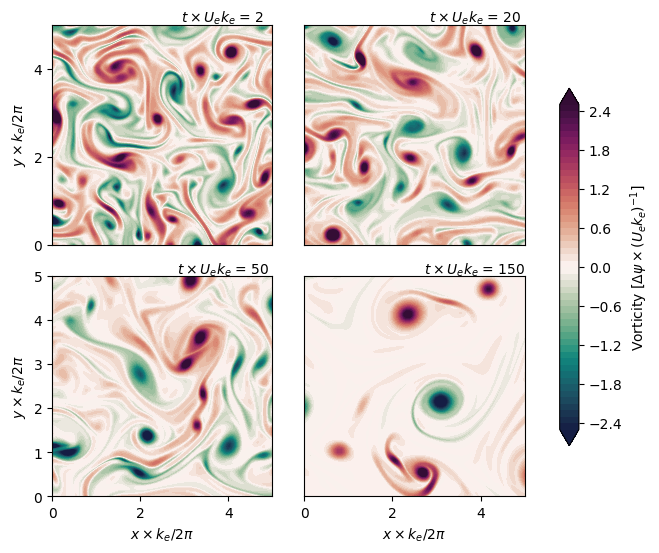
\includegraphics[width=1.\textwidth]{figs/figc1.png}
% \caption{Snapshots of vorticity $\lap\psi$ of a waveless macroturbulence reference solution
%           (standard barotropic QG dynamics). The contours are the same as those of the
%           figures in the main text.}
% \end{figure}
%
% \begin{figure}
% \label{figc2}
% \centering
% 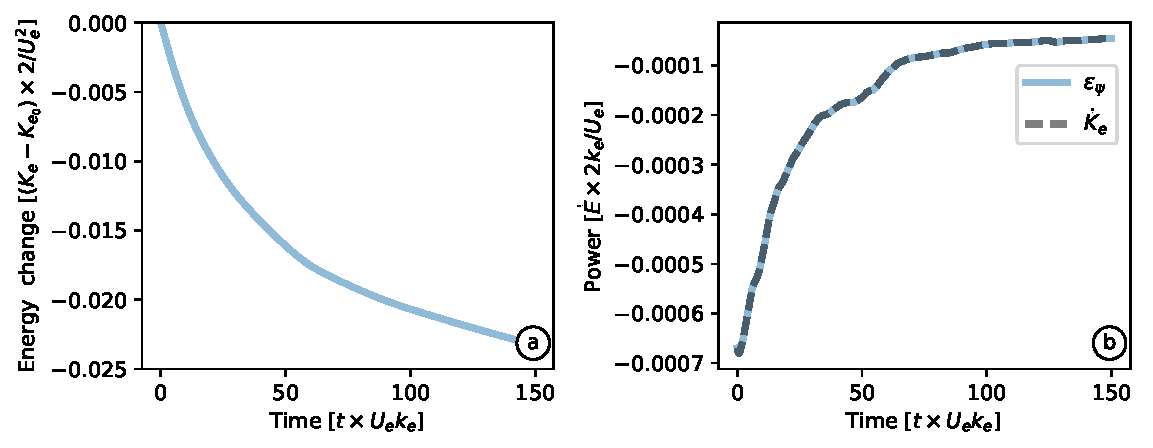
\includegraphics[width=1.\textwidth]{figs/figc2.pdf}
% \caption{(a) The kinetic energy fractional change about initial condition and
%          (b) the energy budget of the waveless macroturbulence reference solution.}
% \end{figure}



\clearpage
\bibliographystyle{jfm}
% Note the spaces between the initials
\bibliography{RochaWagnerYoung}



\end{document}
